%\documentclass[../../tesis.tex]{subfiles}
\documentclass[class=article, crop=false]{standalone}
\usepackage[subpreambles=true]{standalone}
\usepackage{import}
\graphicspath{{images/}}


%
%
%
%
\usepackage{amssymb}
\usepackage{amsmath}
%\usepackage{natbib}
\setcounter{tocdepth}{3}
\usepackage{graphicx}
%\graphicspath{ {Graficos/} }
\usepackage{subfigure}
\usepackage{gensymb}
\usepackage{authblk}
\usepackage{url}
\usepackage[utf8]{inputenc}

\usepackage[spanish]{babel}
\selectlanguage{spanish}
%\usepackage[style=authoryear]{biblatex}

\usepackage{nameref}

\begin{document}
	
	
	
	
	
	
	\section{introducción}
	\info{inclyue estado del arte}
	
	
	\section{Análisis exploratorio de datos}
	
	El análisis exploratorio de la información desagregada a nivel producto implica un mayor nivel de complejidad, dado que se incorpora una nueva dimensión, de alta cardinalidad, al estudio. Dado que la información a nivel de comercio agregado entre países ya fue realizada en el capítulo previo, en este análisis exploratorio se realizará foco en comprender la composición de las canastas exportadoras e importadoras de los países.
	
	Dado que los nomencladores de productos en su nivel desagregado implican una alta cardinalidad, el estudio de su distribución resulta inabarcable. Por ello, tradicionalmente el análisis económico recurre a diferentes niveles de agregación. Para realizar el análisis exploratorio de esta sección recurrimos al nomenclador elaborado por  \cite{molinari2016especializacion} a partir del concepto de \textit{cadenas productivas}. Este nomenclador tiene dos niveles de agregación: Cadenas y Subcadenas (ver Apéndice).
	
		
	La figura \ref{fig:treemaps_global} muestra la distribución de las exportaciones según Cadenas, Subcadenas y Usos, para el promedio mundial durante el período 1996-2016. En \ref{fig:treemaps_global_1} se puede ver que las dos cadenas más importantes son las de Bienes de Capital y Otras Manufacturas, dentro de las cuales las subcadenas que destacan son los equipos eléctricos y de transporte. 	Les sigue la cadena de insumos difundidos, donde destacan los metales y químicos. También son importantes las subcadenas de autopartes, autos, y dentro de la cadena de combustibles, el gas y petróleo. En la figura \ref{fig:treemaps_global_2} las cadenas se subdividen según el uso que se le da a los productos: Productos Primarios, Bienes de Capital, etc (ver Apéndice). Vale mencionar que la cadena Bienes de Capital no incluye exclusivamente productos de este tipo, tal como se observa en la figura, dado que las cadenas hacen referencia a las Cadenas de valor \citep{humphrey2000governance}, es decir a la rama de la producción a la que pertenecen los productos del final de la cadena. Allí podemos observar que en la cadena de Otras manufacturas destacan los productos semiterminados y bienes de consumo, mientras que en las cadena de Bienes de capital destacan su homónimo y las partes y componentes. A su vez en la cadena de insumos difundidos destacan los productos semiterminados ampliamente, mientras que en la industria automotriz se exportan mayoritariamente partes y componentes. 
	
	\begin{figure}
		\centering
		\subfigure[Cadenas y Subcadenas]{\label{fig:treemaps_global_1}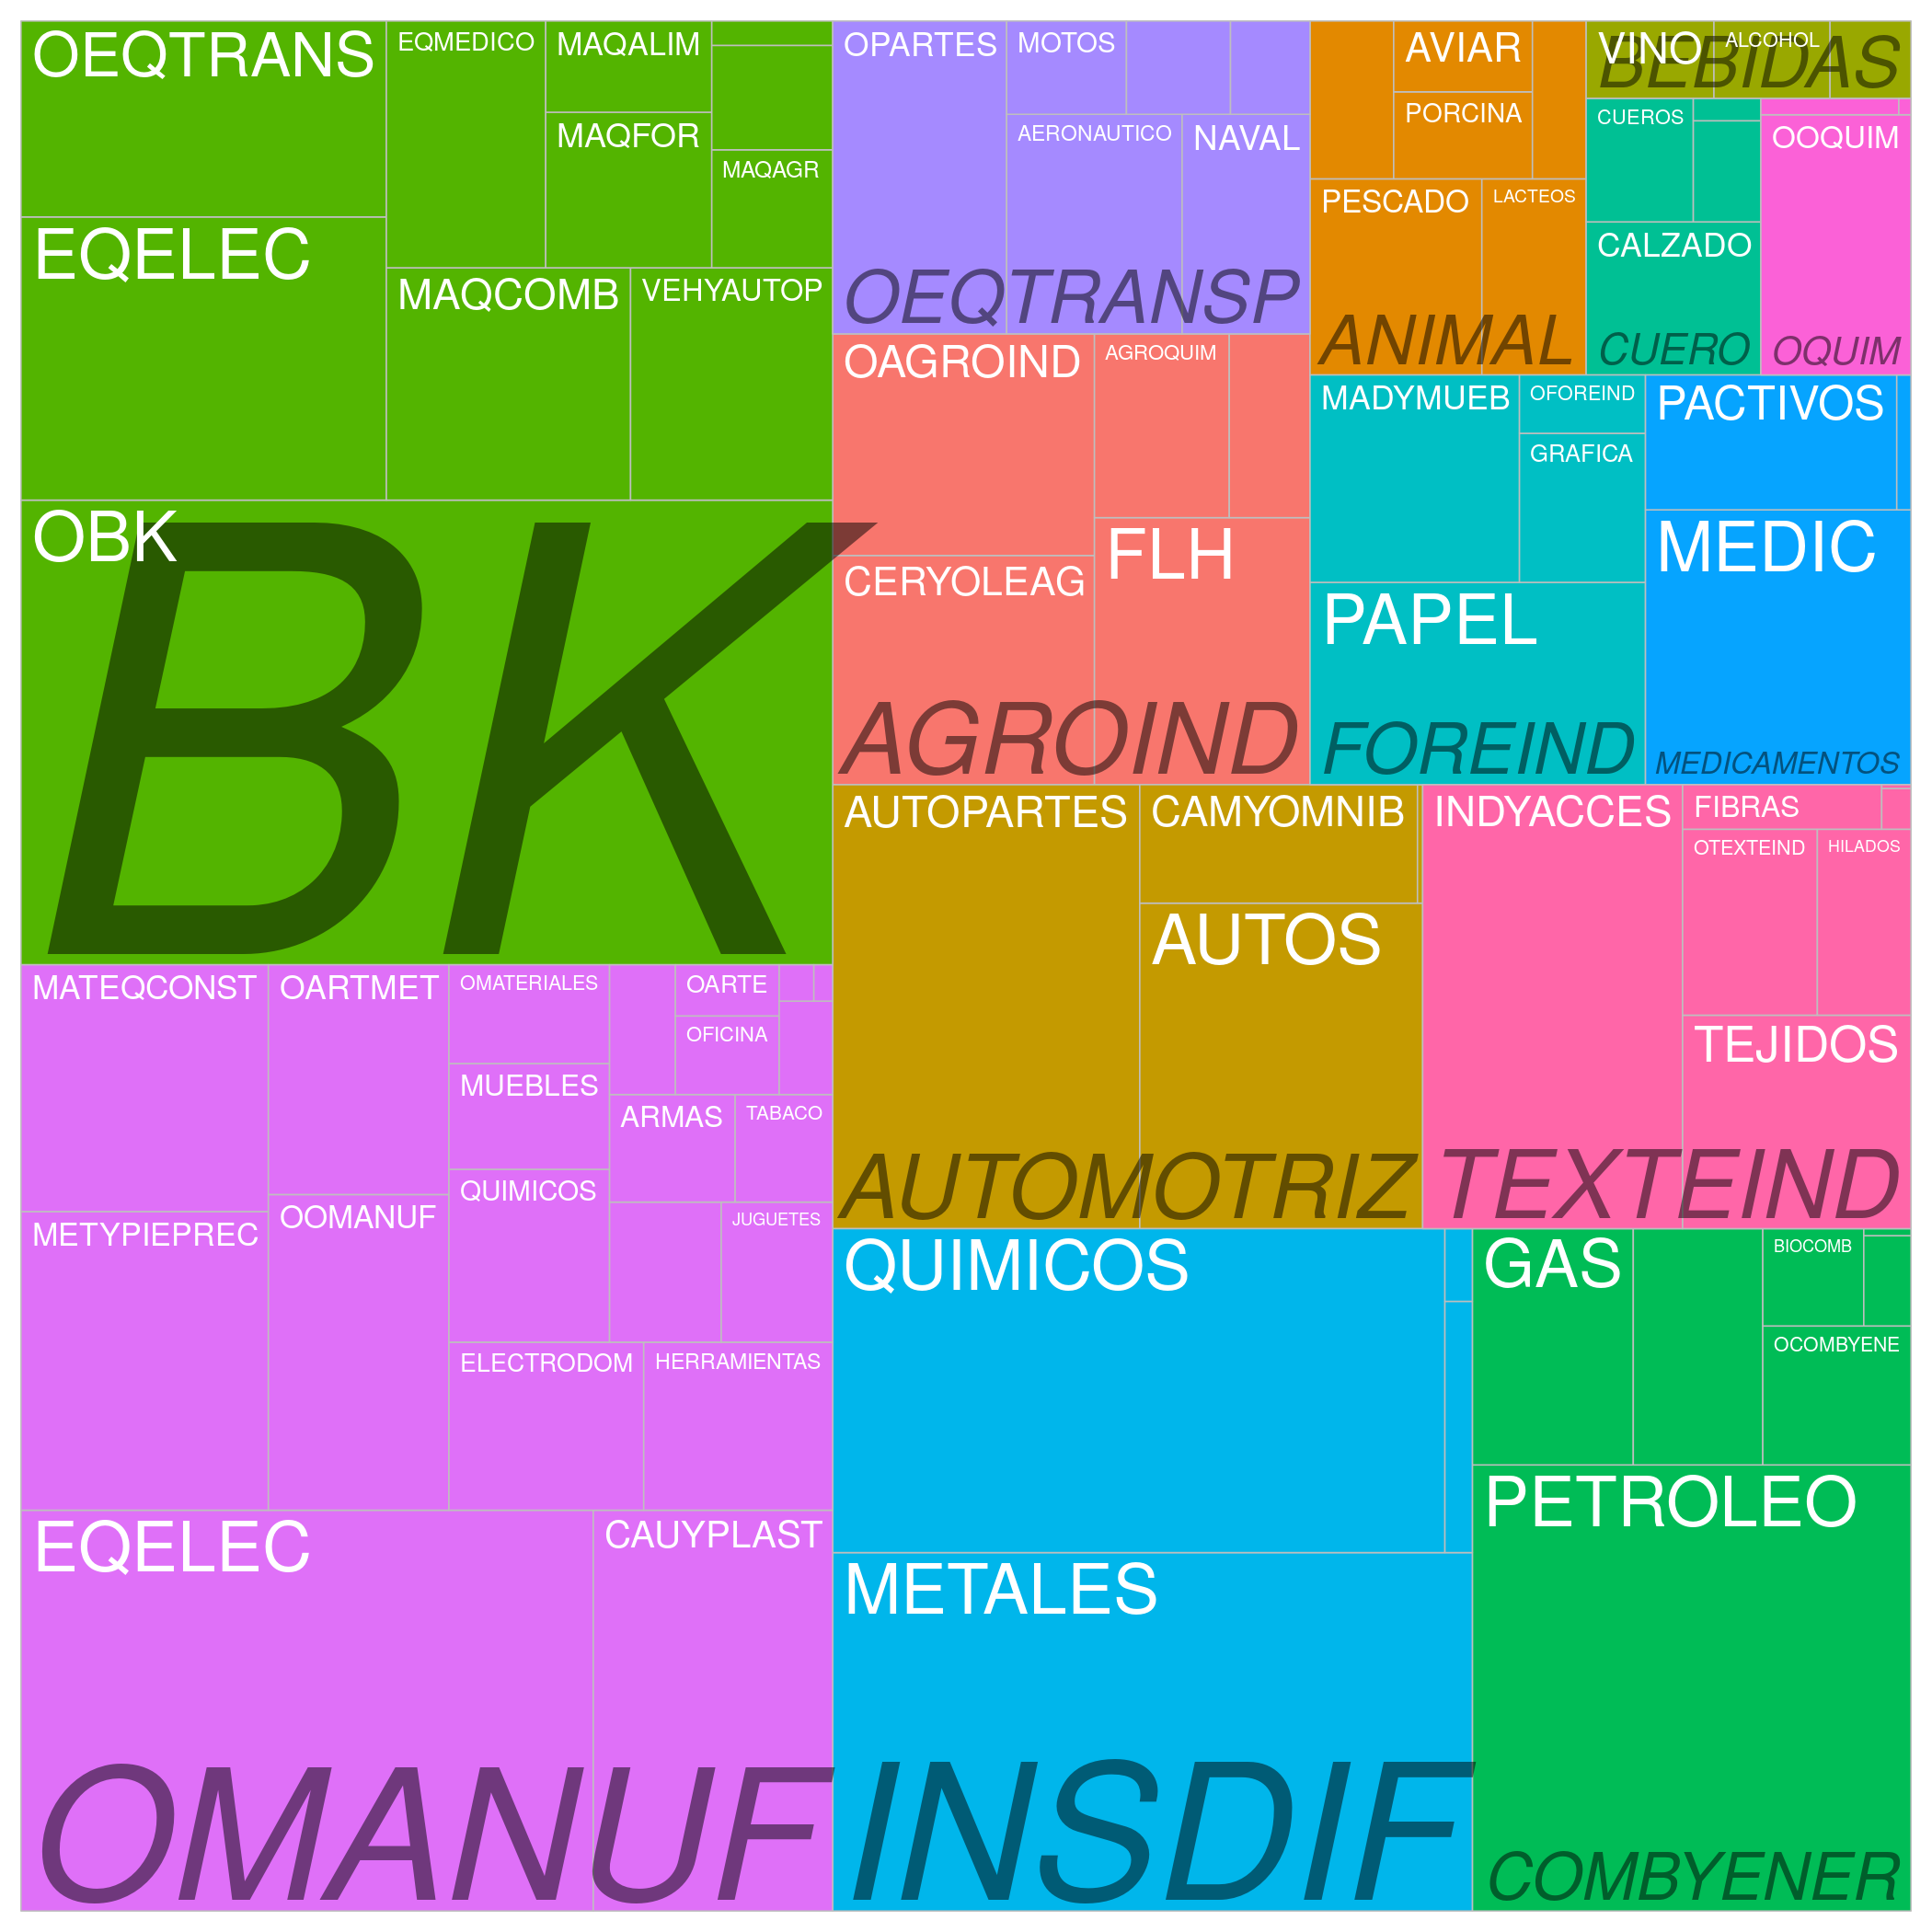
\includegraphics[width=.65\linewidth]{treemap_cadsubcad.png}}
		\subfigure[Cadenas y Usos]{\label{fig:treemaps_global_2}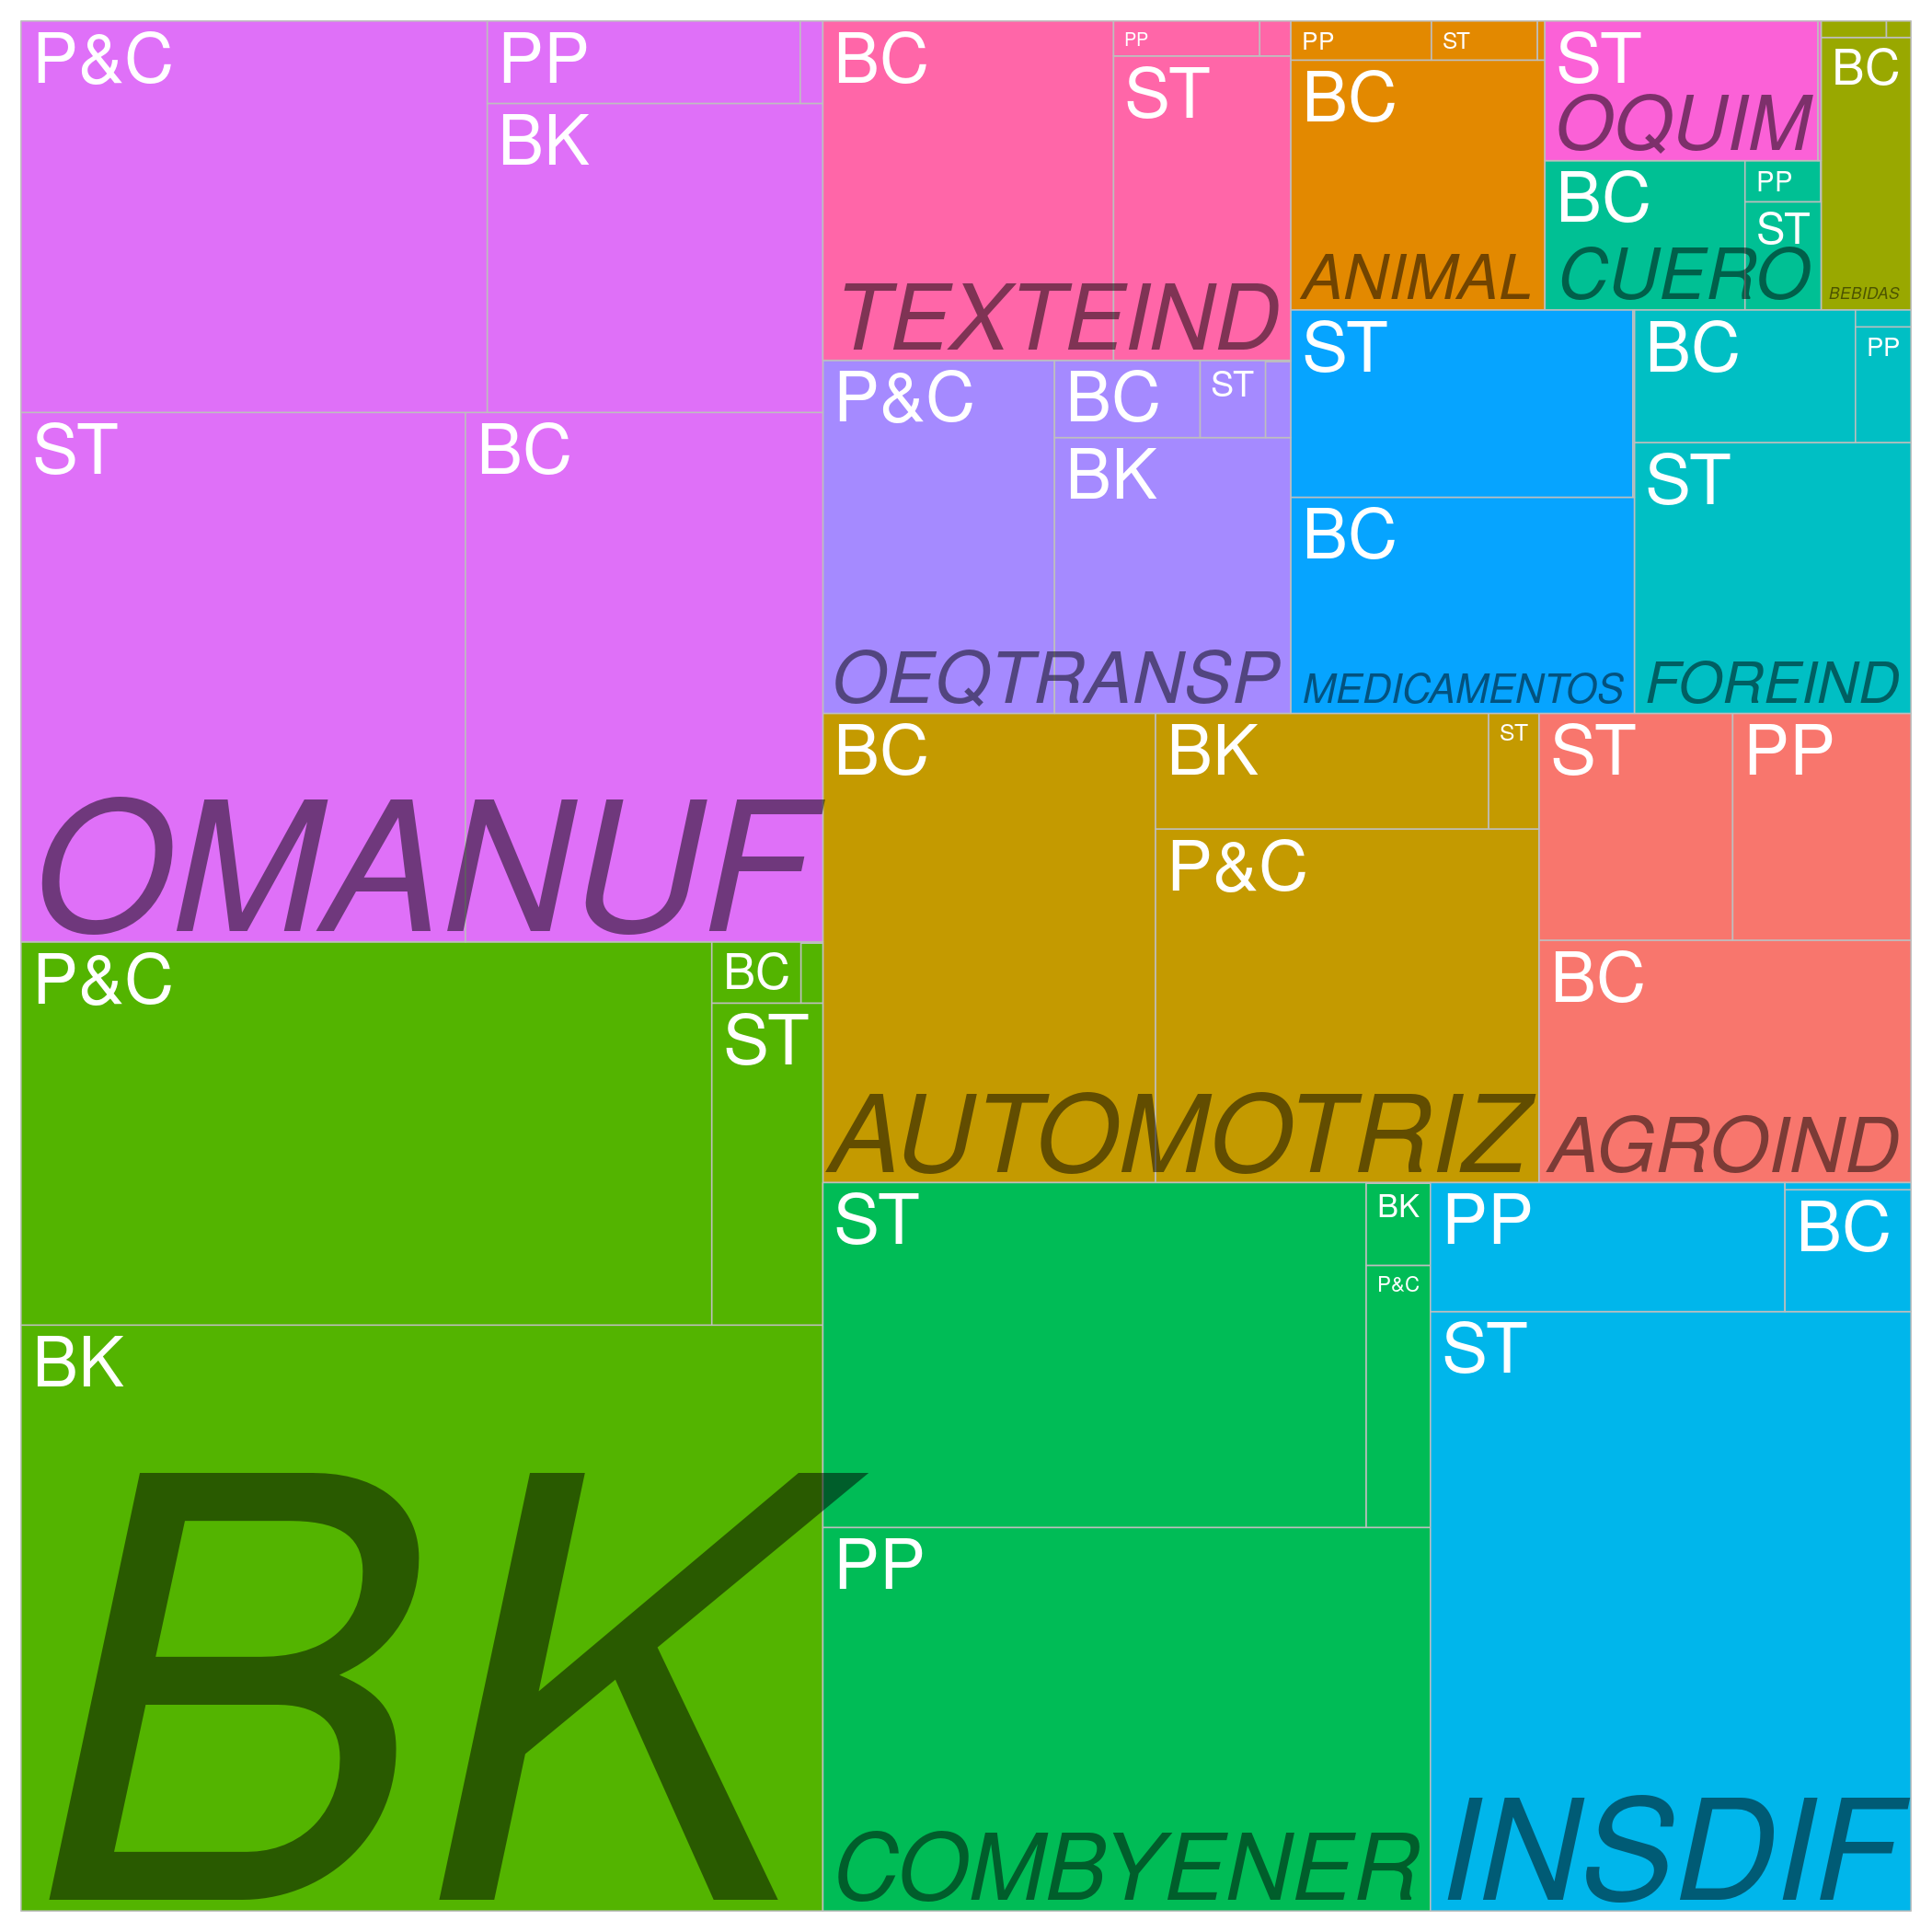
\includegraphics[width=.65\linewidth]{treemap_usos.png}}
		\caption{Treemaps por tipos de productos. Exportaciones. 1996-2016. Total mundial}
		\label{fig:treemaps_global}
	\end{figure}
	
	
	
	La figura \ref{fig:treemaps_global_paises} muestra la distribución de las exportaciones e importaciones según continente y país exportador, para el promedio 1996-2016. Allí destaca el mayor volumen de exportaciones que importaciones de Asia, y el mayor volumen de importaciones que exportaciones de Estados Unidos, siguiendo las mismas conclusiones que el capítulo 2. 
	
	
	\begin{figure}
		\centering
		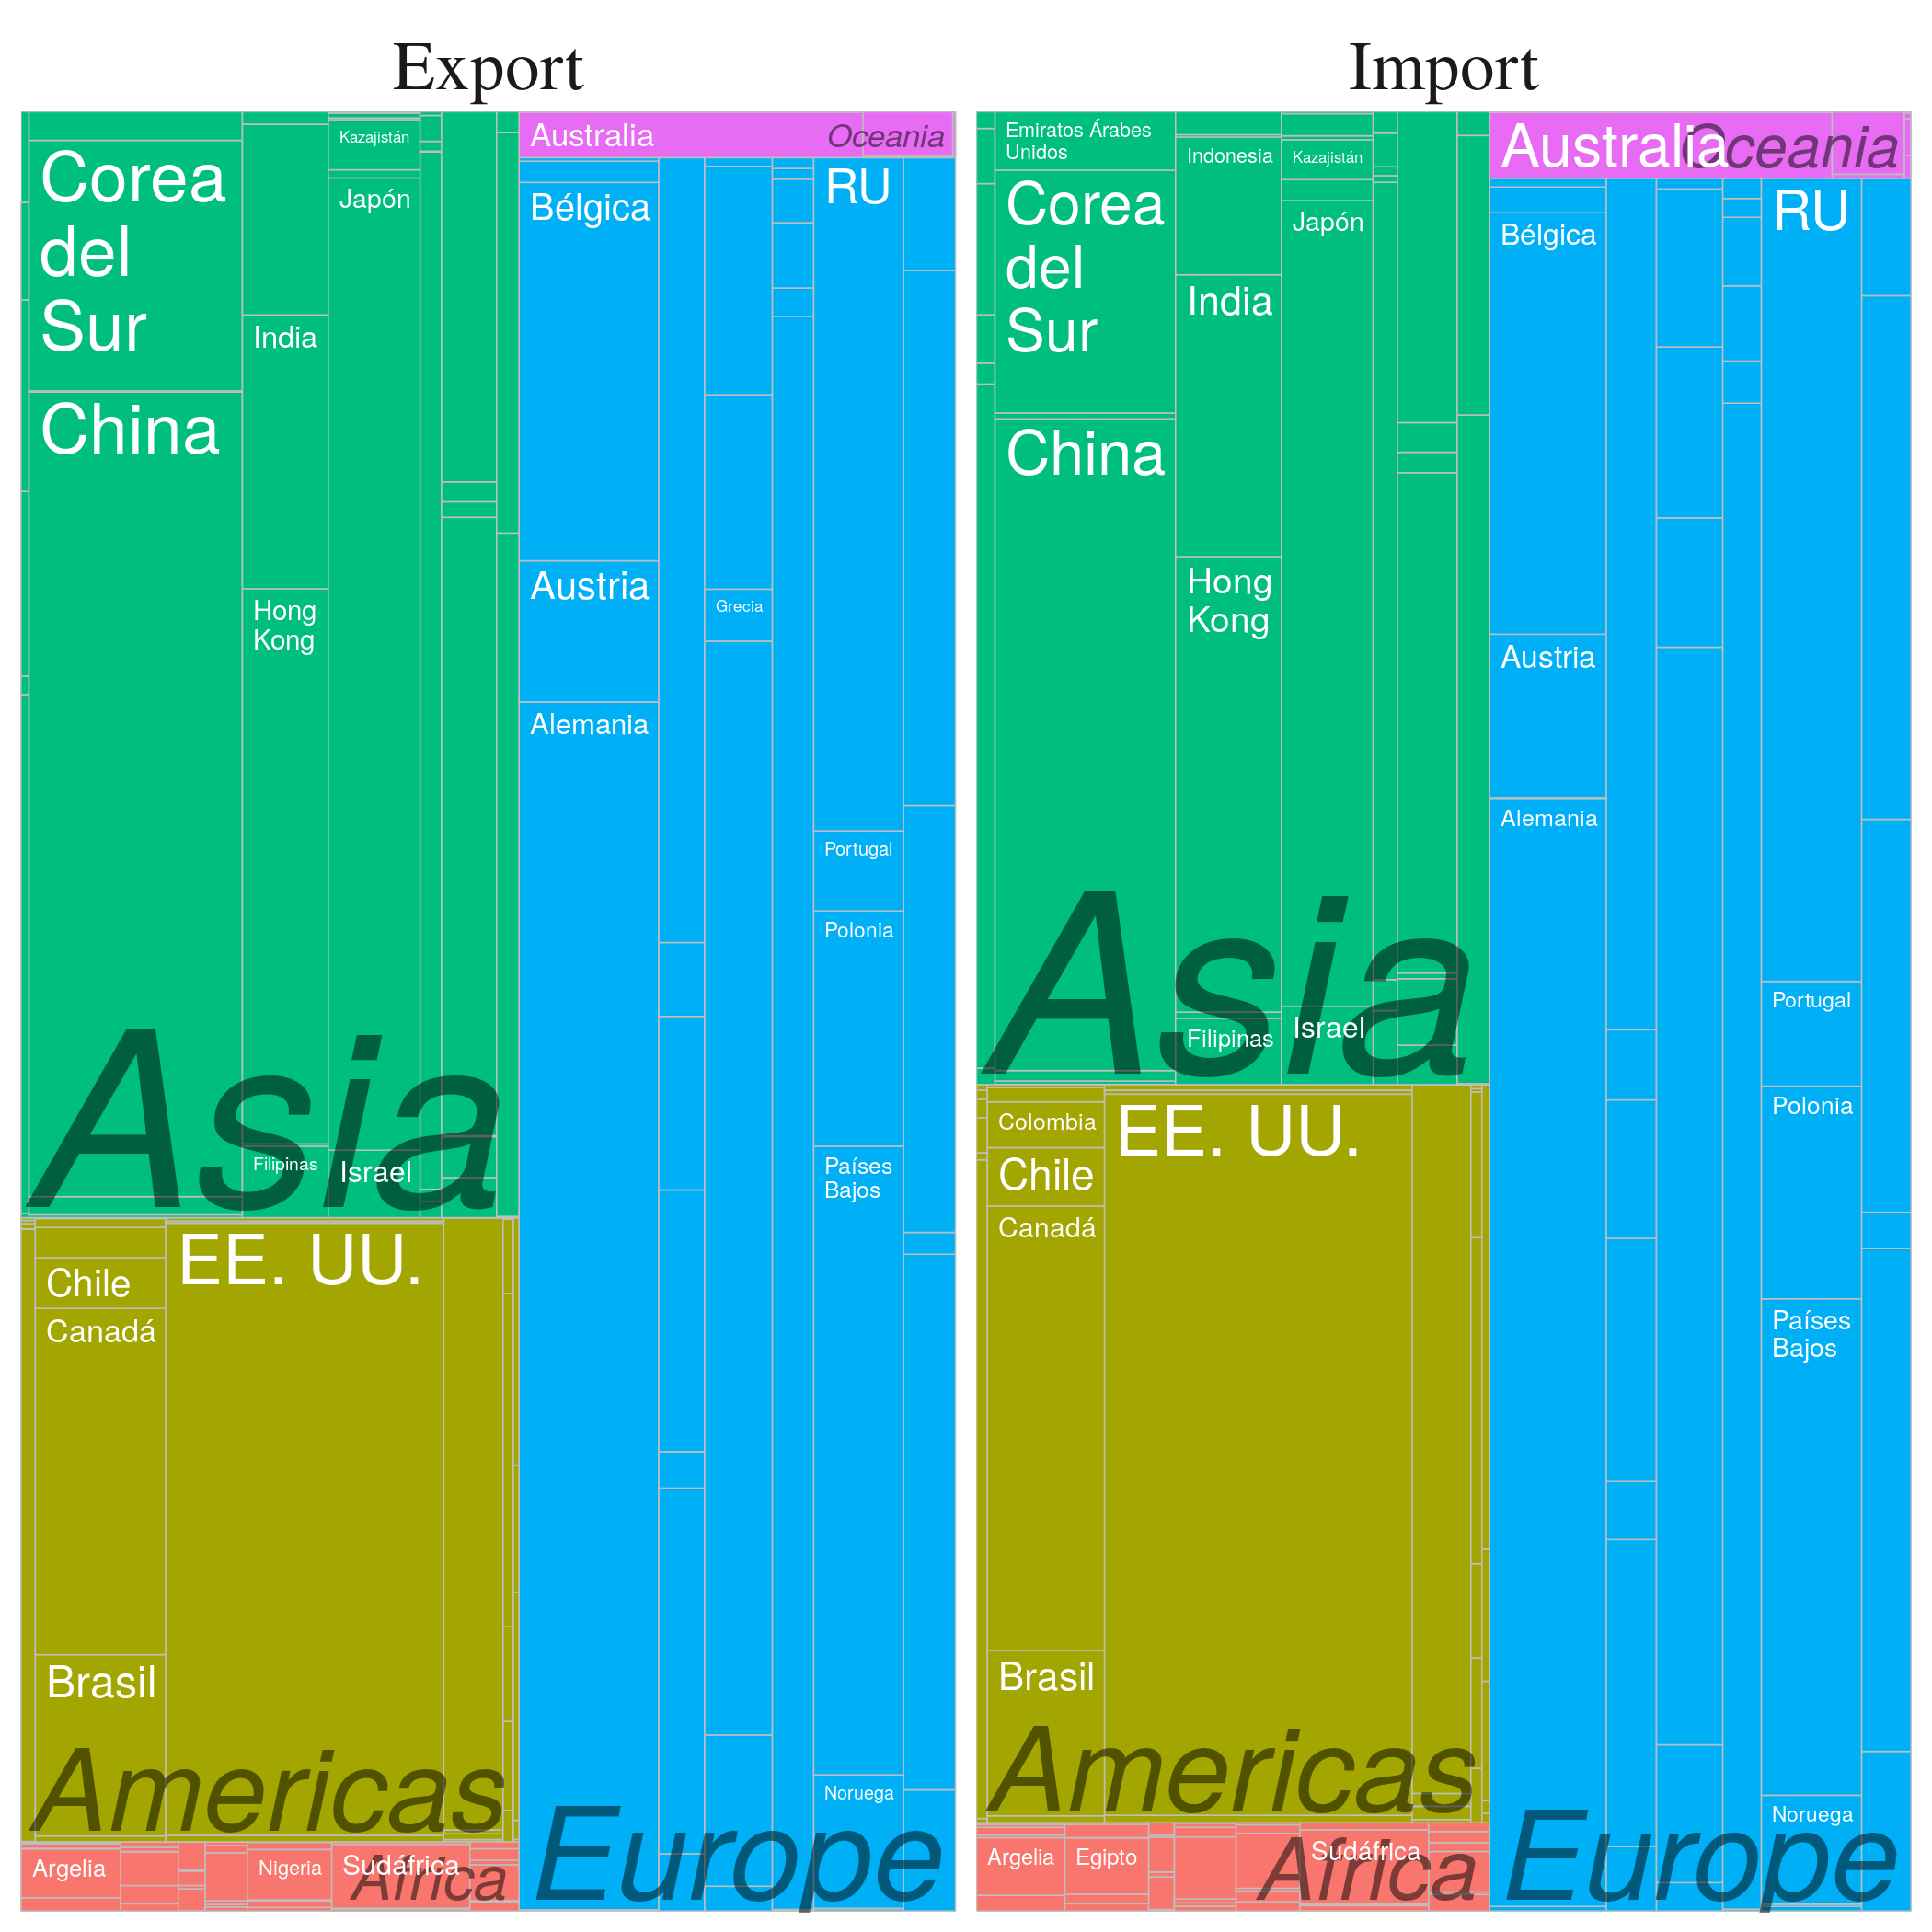
\includegraphics[width=.75\textwidth]{treemap_paises}
		\caption{Treemaps por Continentes y países. 1996-2016. Total mundial}
				\label{fig:treemaps_global_paises}
	\end{figure}
	
	
	Sin embargo, la riqueza en el análisis a nivel producto se encuentra en comprar la distinta composición de la balanza comercial de los países. Ya sea la diferencia entre la composición de sus exportaciones respecto de sus importaciones, como de estos elementos respecto de otros países o regiones. Dado que dicho análisis implica la comparación de una multiplicidad de treemaps, se decidió elaborar una herramienta interactiva para el análisis. La misma fue elaborada utilizando la librería \textit{shiny} \citep{Chang2018} y se encuentra disponible en \hyperlink{https://treemaps.shinyapps.io/treemaps/}{https://treemaps.shinyapps.io/treemaps/}. Dados los límites del servidor y el interés de estudiar la herramienta para un caso específico, el análisis se centra en el caso latinoamericano, tanto para el subcontinente en conjunto como para los países que lo integran. El objeto de análisis es estudiar las posibilidades de integración regional de la producción, y para ello analizar el comportamiento diferencial de las canastas exportadoras e importadoras de los países latinoamericanos cuando comercian entre sí respecto de su comercio con el resto del mundo. A su vez, dada la importancia del comercio de esta región con China, se decidió dividir la información del resto del mundo exceptuando a China y este país de forma individual.
	
	En la figura \ref{fig:treemaps_sudamerica_cadsubcad} se pueden observar los treemaps de cadenas y subcadenas para 2016 del total de los países sudamericanos, según su destino. En la figura \ref{fig:treemaps_sudamerica_cadsubcad_1} se ve como la canasta exportadora de los países latinoamericanos varía según si su destino se encuentra dentro o fuera de la región, y en particular si son exportaciones hacia China. En particular, el comercio intra-regional tiene un componente importante de bienes de capital, y del sector automotriz, ya sean autos terminados o autopartes. Por su parte, en el comercio con el resto del mundo estos componentes cumplen un rol secundario, mientras que se destacan las cadenas agroindustriales, de combustibles e insumos industriales. Respecto del resto del mundo, el comercio con China resalta por las exportaciones de la subcadena de biocombusitbles, cereales y oleaginosas y Metales. 
	Las importaciones de estos mismos países se pueden observar en la figura \ref{fig:treemaps_sudamerica_cadsubcad_2}. Naturalmente los treemaps de las exportaciones e importaciones son muy similares, ya que la única diferencia es el país que registra la operación. Sin embargo, en las importaciones del resto del mundo destacan las cadenas automotriz y de bienes de capital. A su vez, resulta de interés el cambio de composición de las cadenas: Mientras que las exportaciones de insumos industriales hacia el resto del mundo son mayoritariamente metales, en las importaciones destacan los productos químicos. Por su parte, mientras que en la cadena de otras manufacturas se exportan hacia el resto del mundo metales y piedras preciosas, se importan dentro de esta cadena equipos eléctricos. A su vez, del resto del mundo se importan medicamentos, aunque este rubro no aparece en el treemap de las exportaciones. Cabe destacar que la región exporta e importa petróleo hacia el resto del mundo, aunque el comercio intrarregional de este producto es menor. Existe, por lo tanto, una potencialidad de integración comercial dentro de la región para este producto en particular. 
	El comercio con China esta particularmente orientado a la venta de materias primas y la compra de productos industriales. Destacan especialmente las exportaciones de cereales y oleaginosas, biocombustibles y metales; mientras que se importan equipos eléctricos, bienes de capital, calzados y químicos. 
	

\begin{figure}
	\centering
	\subfigure[Exportaciones]{\label{fig:treemaps_sudamerica_cadsubcad_1}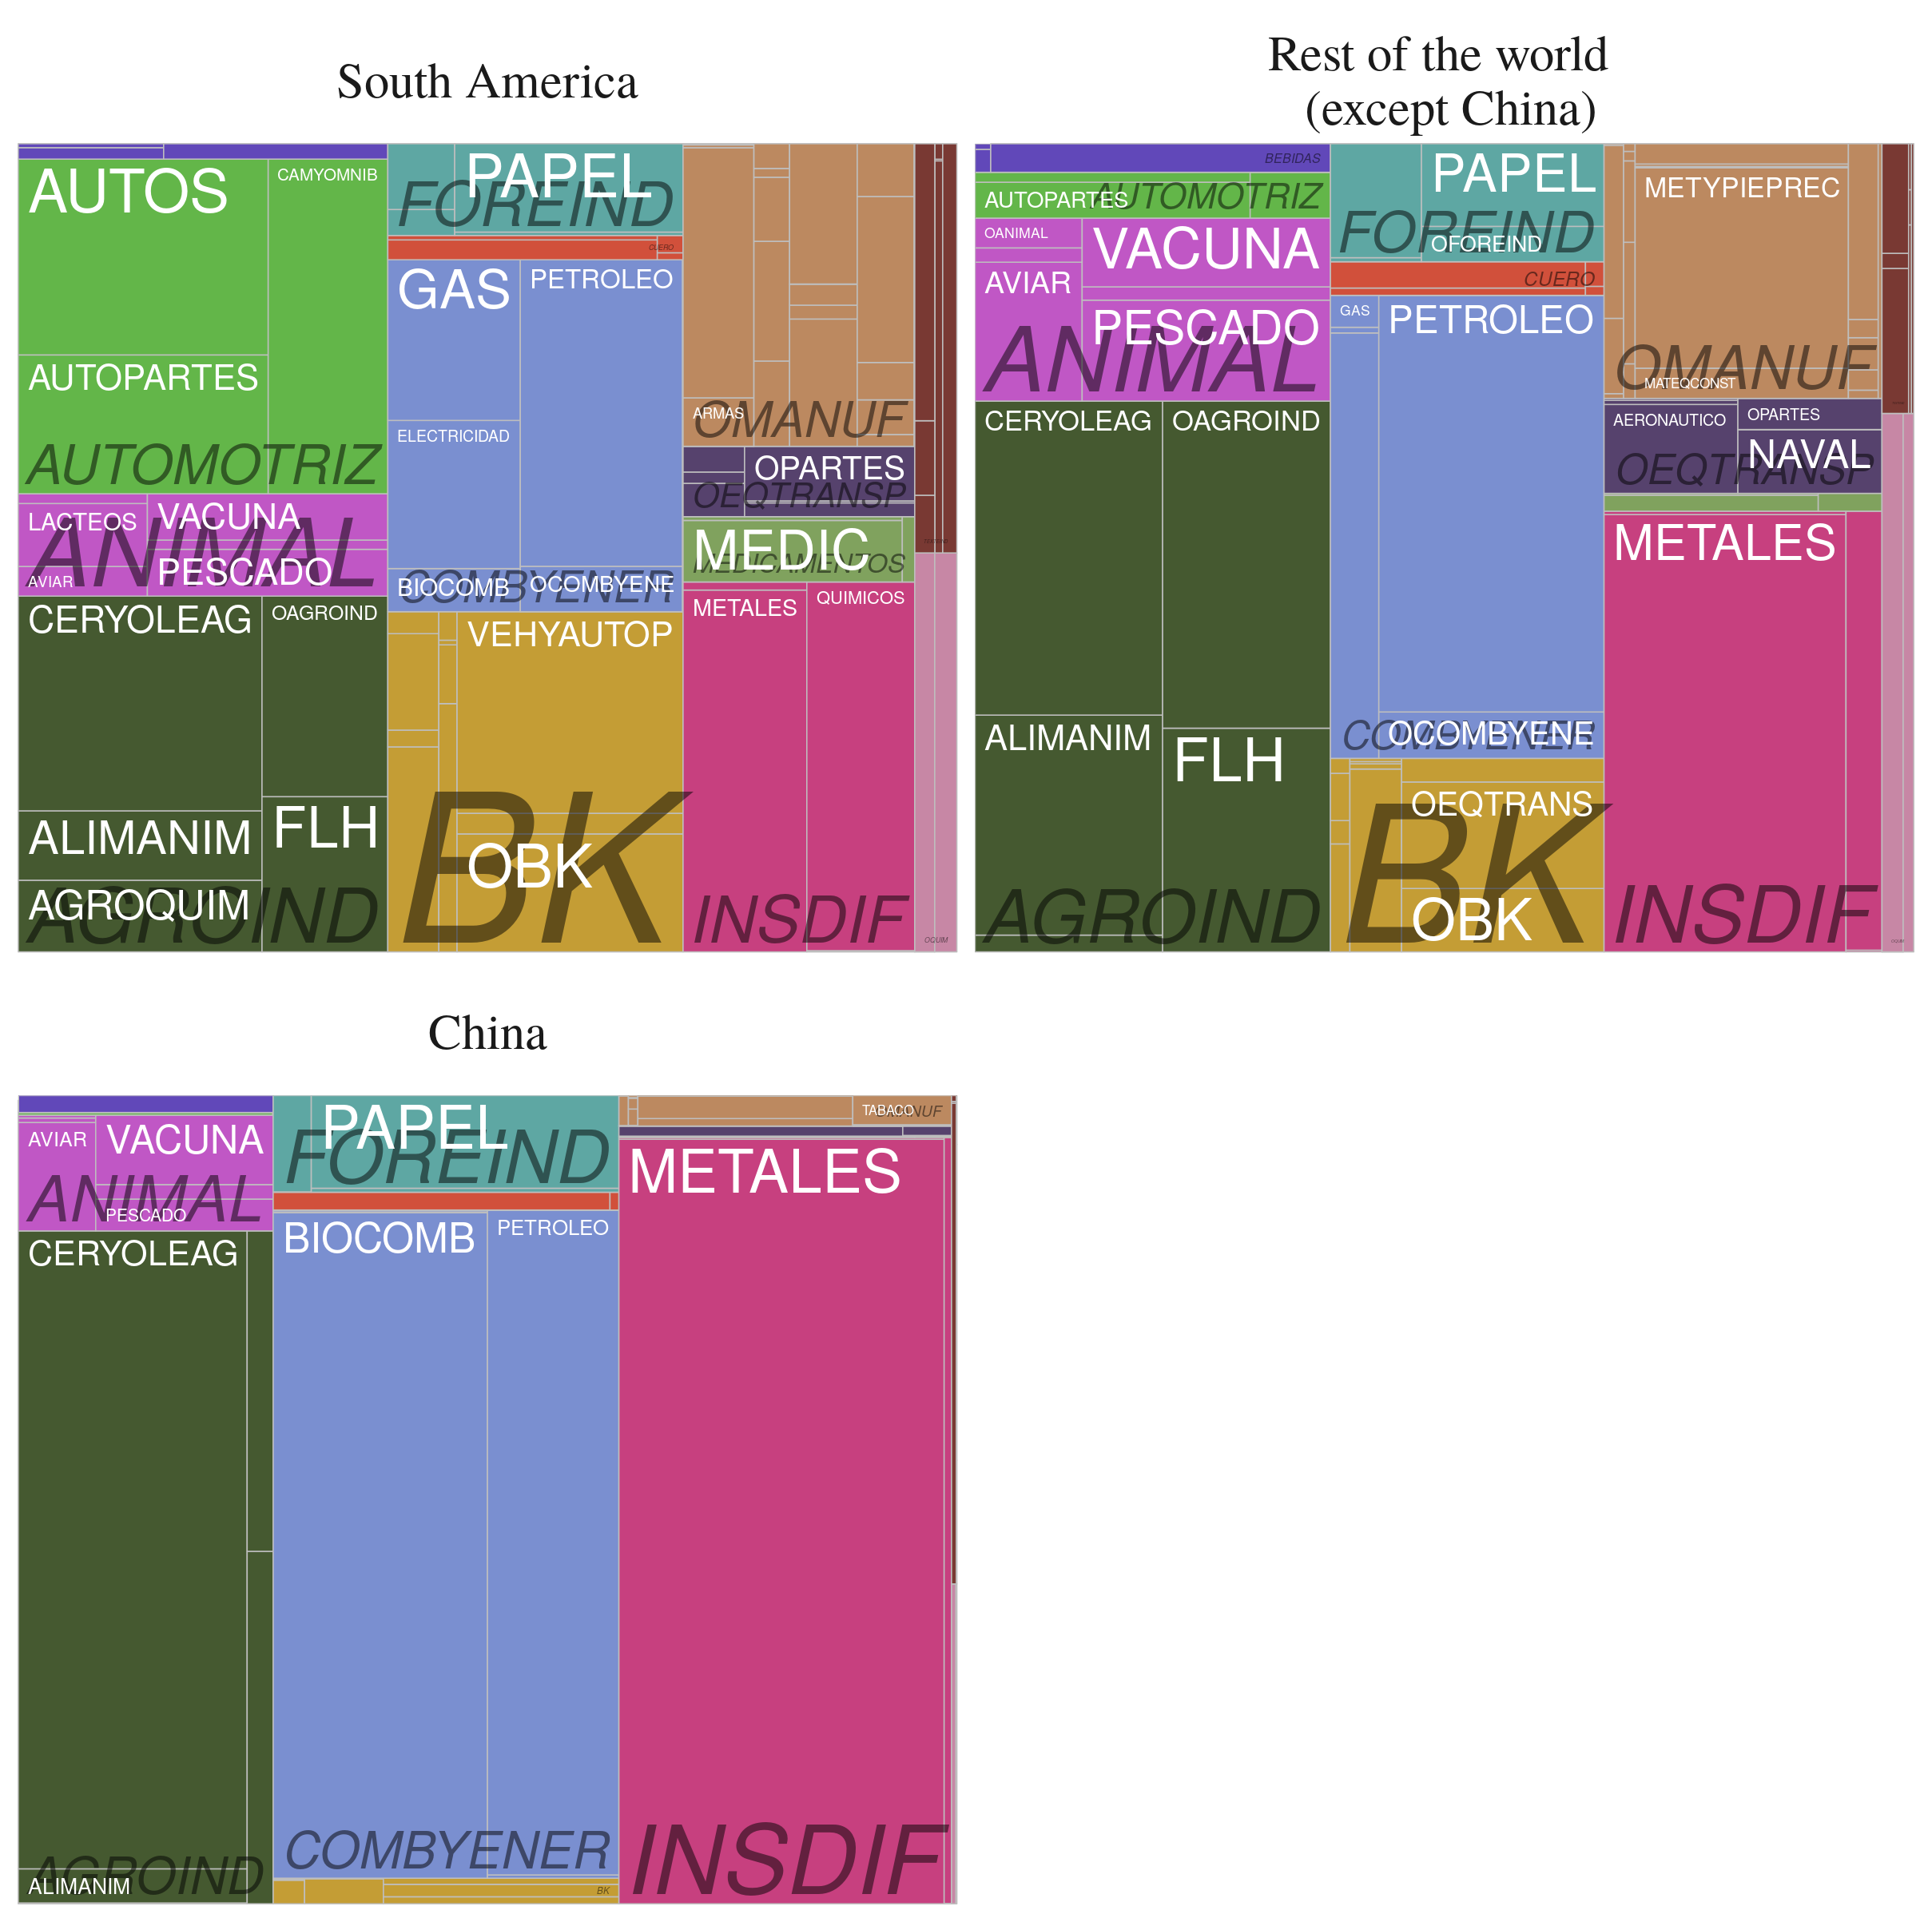
\includegraphics[width=.75\linewidth]{treemaps_cadsubcad2016}}
	\subfigure[Importaciones]{\label{fig:treemaps_sudamerica_cadsubcad_2}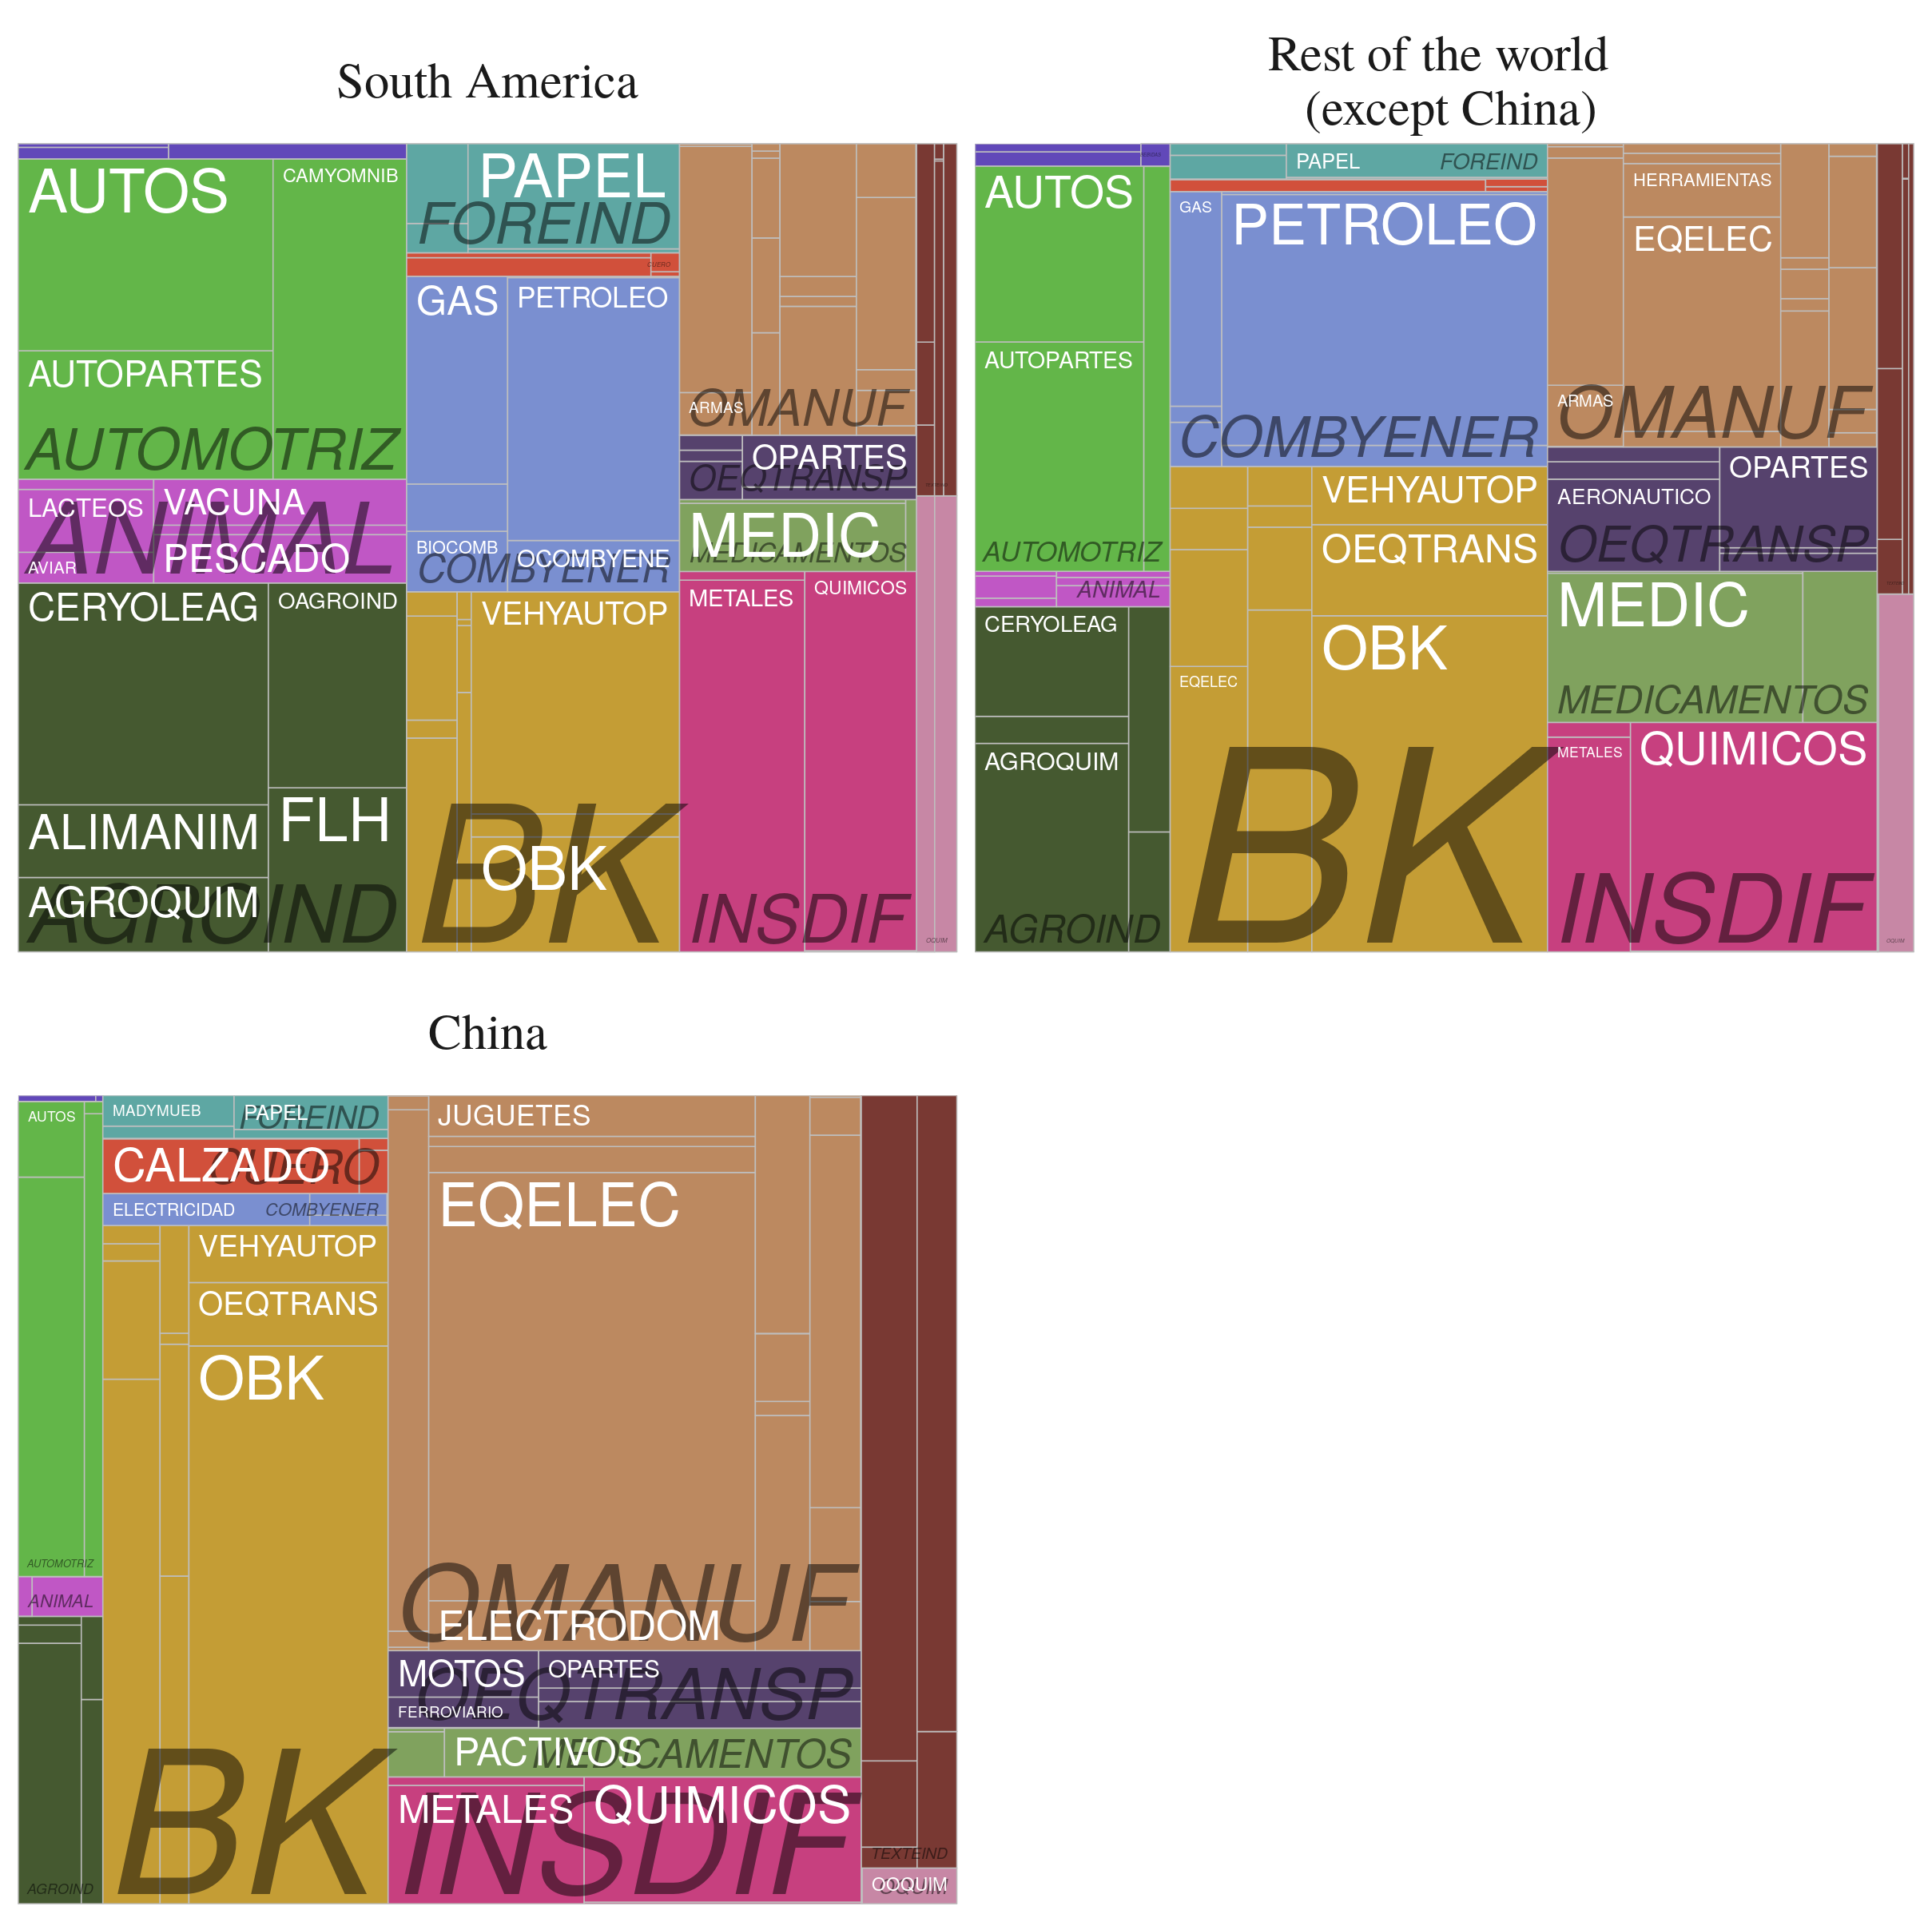
\includegraphics[width=.75\linewidth]{treemaps_cadsubcad2016_impos}}
	\caption{Treemaps de Cadenas y Subcadenas.2016. Total Latinoamérica}
	\label{fig:treemaps_sudamerica_cadsubcad}
\end{figure}


La figura \ref{fig:treemaps_sudamerica_usos} muestra los treemaps exclusivamente según los usos de los productos, para el total de la región, según su destino, en el año 2016. En \ref{fig:treemaps_sudamerica_usos_1} se puede observar las exportaciones. Los usos de los productos exportados varían fuertemente según su destino. Los productos semiterminados constituyen la mayoría de las exportaciones tanto hacia el interior de la región, como con el resto del mundo. Sin embargo, mientras que los bienes de consumo resultan de particular importancia dentro de la región, los productos primarios lo son respecto del resto del mundo. El comercio con china destaca esta tendencia, donde la mayoría de las exportaciones provienen de productos primarios. En \ref{fig:treemaps_sudamerica_usos_2} se observa la distribución de las importaciones según su uso. Allí se ve que las importaciones de productos semiterminados desde el resto del mundo supera a las exportaciones, si se lo compara con \ref{fig:treemaps_sudamerica_usos_1}. A su vez, prácticamente no se exportan productos primarios, pero sí partes y componentes, y bienes de capital. El comercio con China se encuentra equitativamente distribuido entre bienes de capital, productos semiterminados, de consumo y partes y componentes. Es notorio que no se importa prácticamente productos primarios, aunque estos constituyen la base de las exportaciones a dicho país. 

\begin{figure}
	\centering
	\subfigure[Exportaciones]{\label{fig:treemaps_sudamerica_usos_1}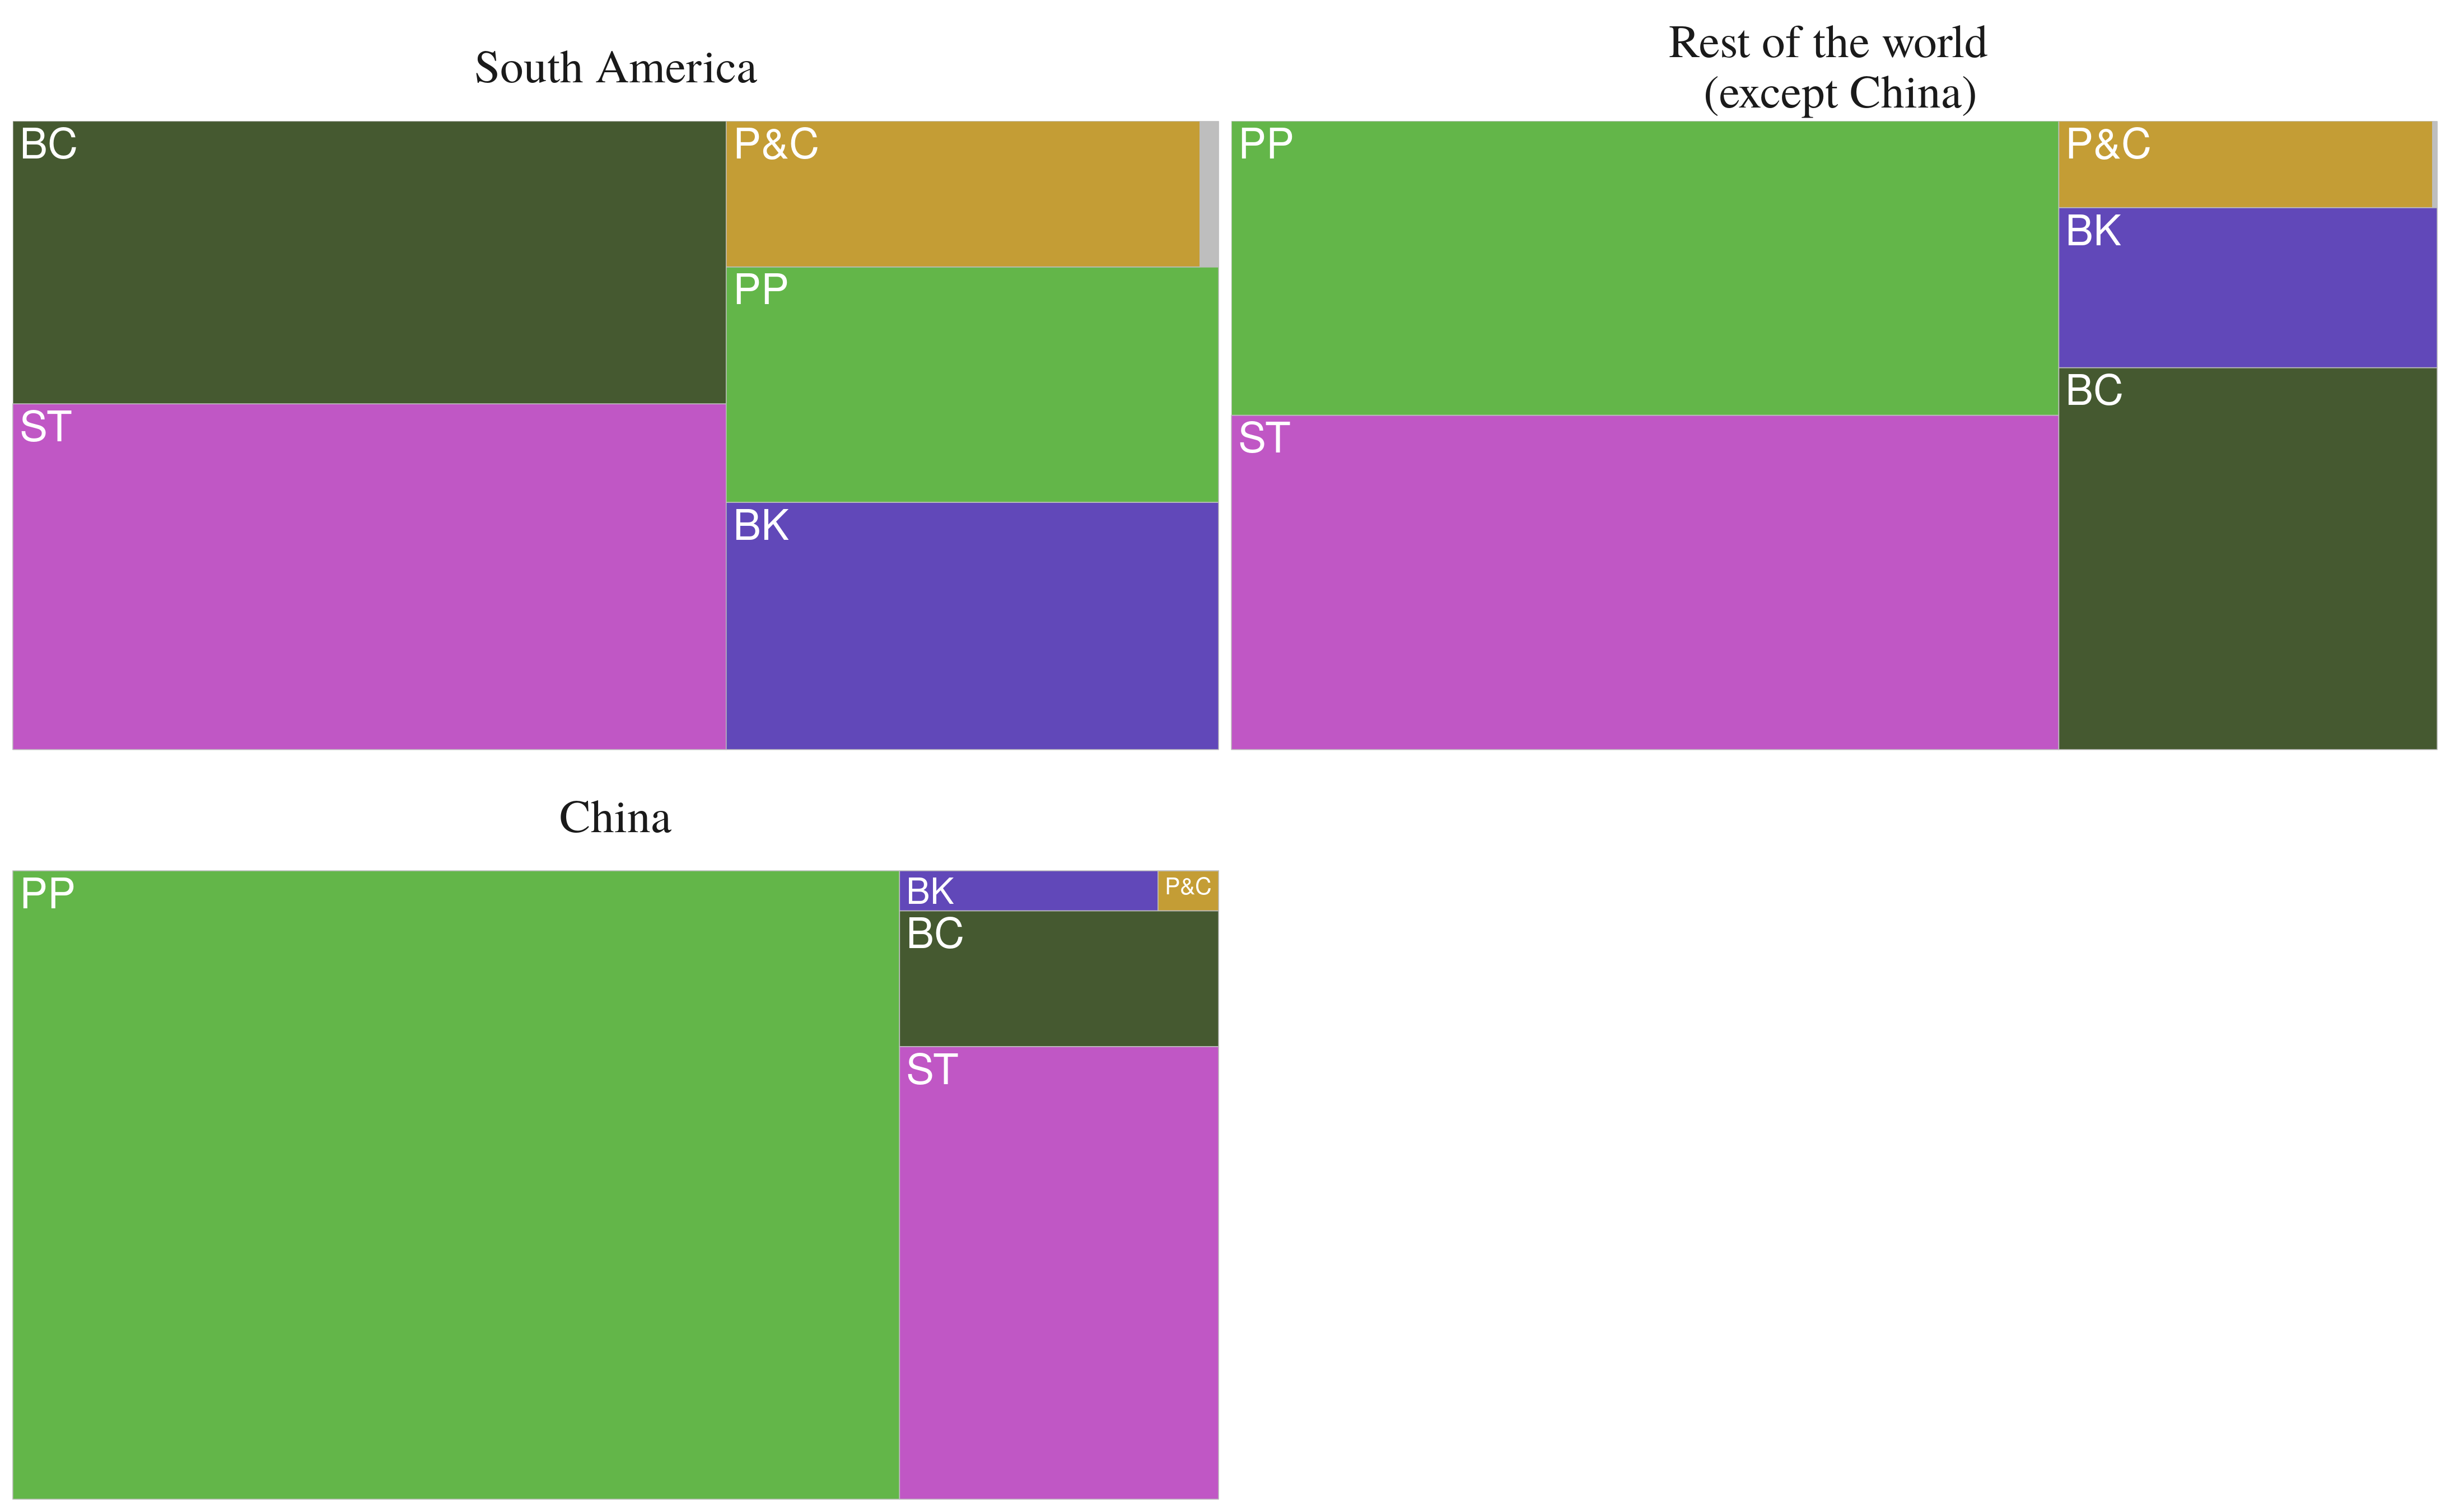
\includegraphics[width=.75\linewidth]{treemaps_usos2016}}
	\subfigure[Importaciones]{\label{fig:treemaps_sudamerica_usos_2}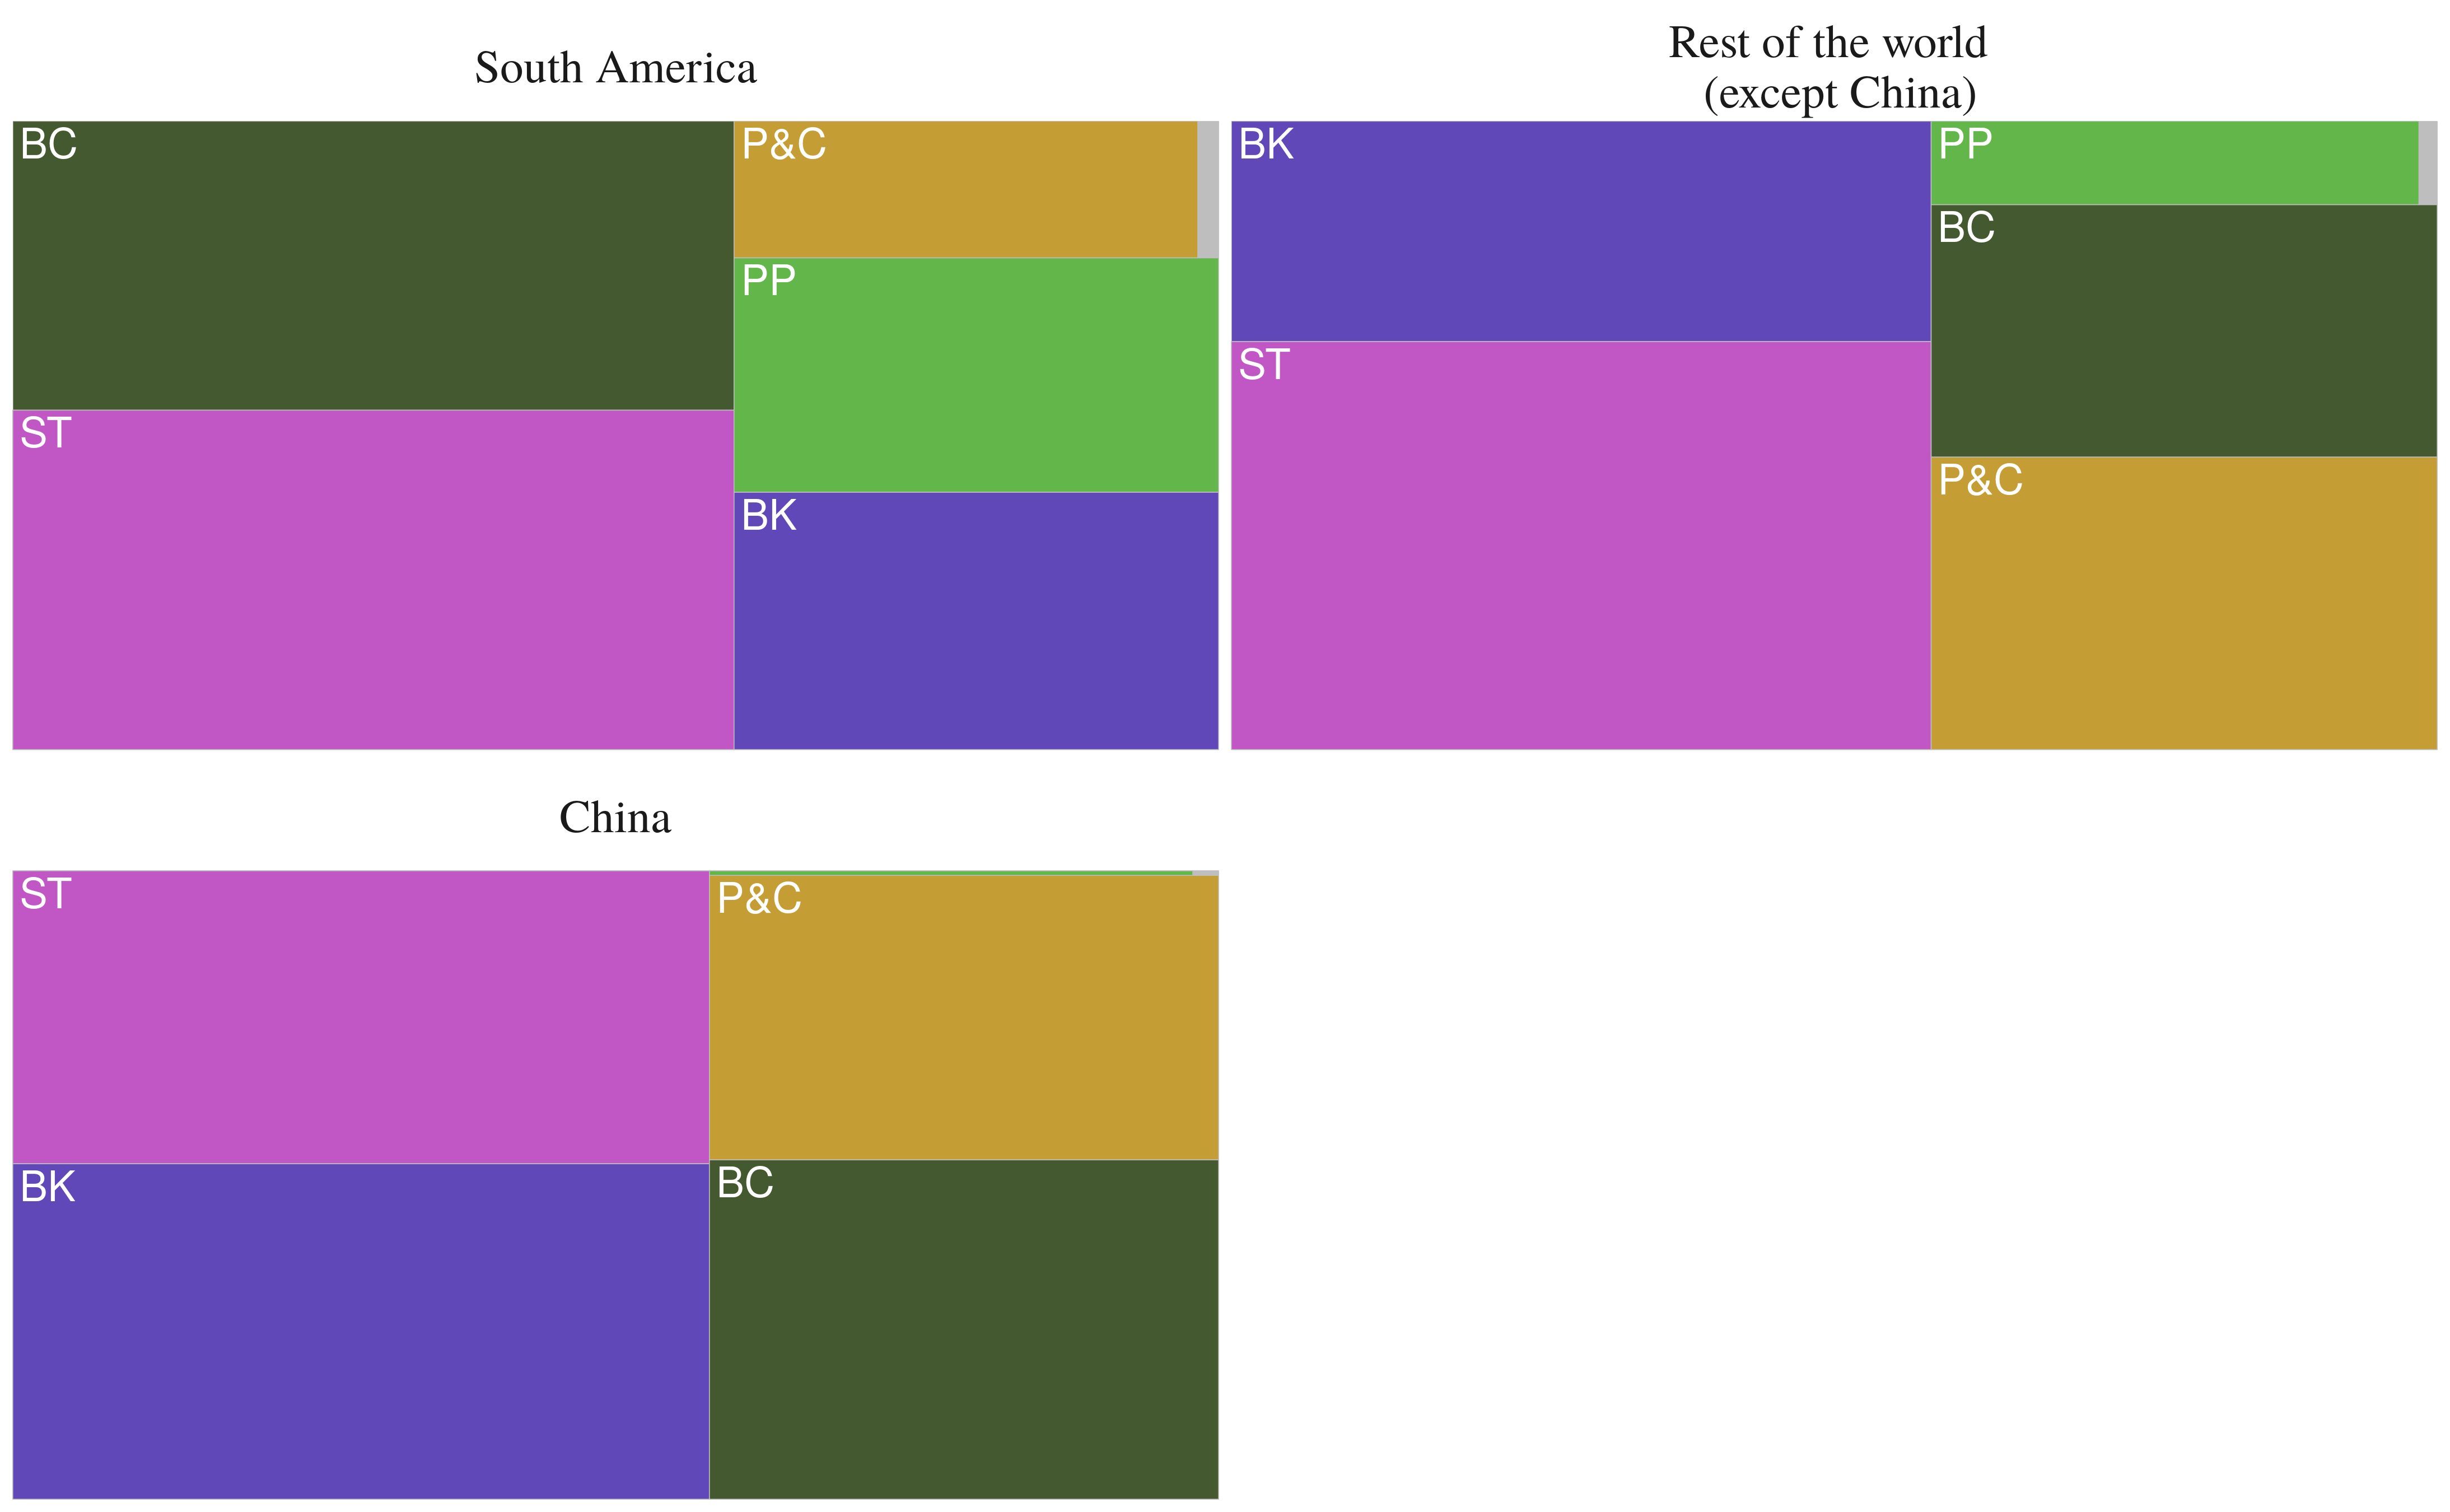
\includegraphics[width=.75\linewidth]{treemaps_usos2016_impos}}
	\caption{Treemaps de Cadenas y Usos.2016. Total Latinoamérica}
	\label{fig:treemaps_sudamerica_usos}
\end{figure}




En la figura \ref{fig:treemaps_sudamerica_destino} se observa la distribución de los socios comerciales de Sudamérica en el 2016. Esto es, los países destino de las exportaciones y origen de las importaciones. En \ref{fig:treemaps_sudamerica_destino_1} se excluye al resto del mundo y China, para observar la distribución interna del comercio. Naturalmente Brasil es el mayor socio comercial interno, para ambos tipos de flujo comercial, aunque su importancia es mucho mayor como exportador que como importador, dado que es el origen del 40\% de las importaciones de los demás países, y el destino del 25\% de las exportaciones. 
En la figura \ref{fig:treemaps_sudamerica_destino_2} se puede observar el mismo gráfico, pero incluyendo al resto del mundo. Allí se ve que tanto las exportaciones como importaciones hacia el resto del mundo exceptuando a China constituyen más de un 60\% del comercio, y China exclusivamente representa casi un 20\% del comercio de la región, superando ampliamente a Brasil. 

\begin{figure}
	\centering
	\subfigure[Excluyendo Resto del Mundo]{\label{fig:treemaps_sudamerica_destino_1}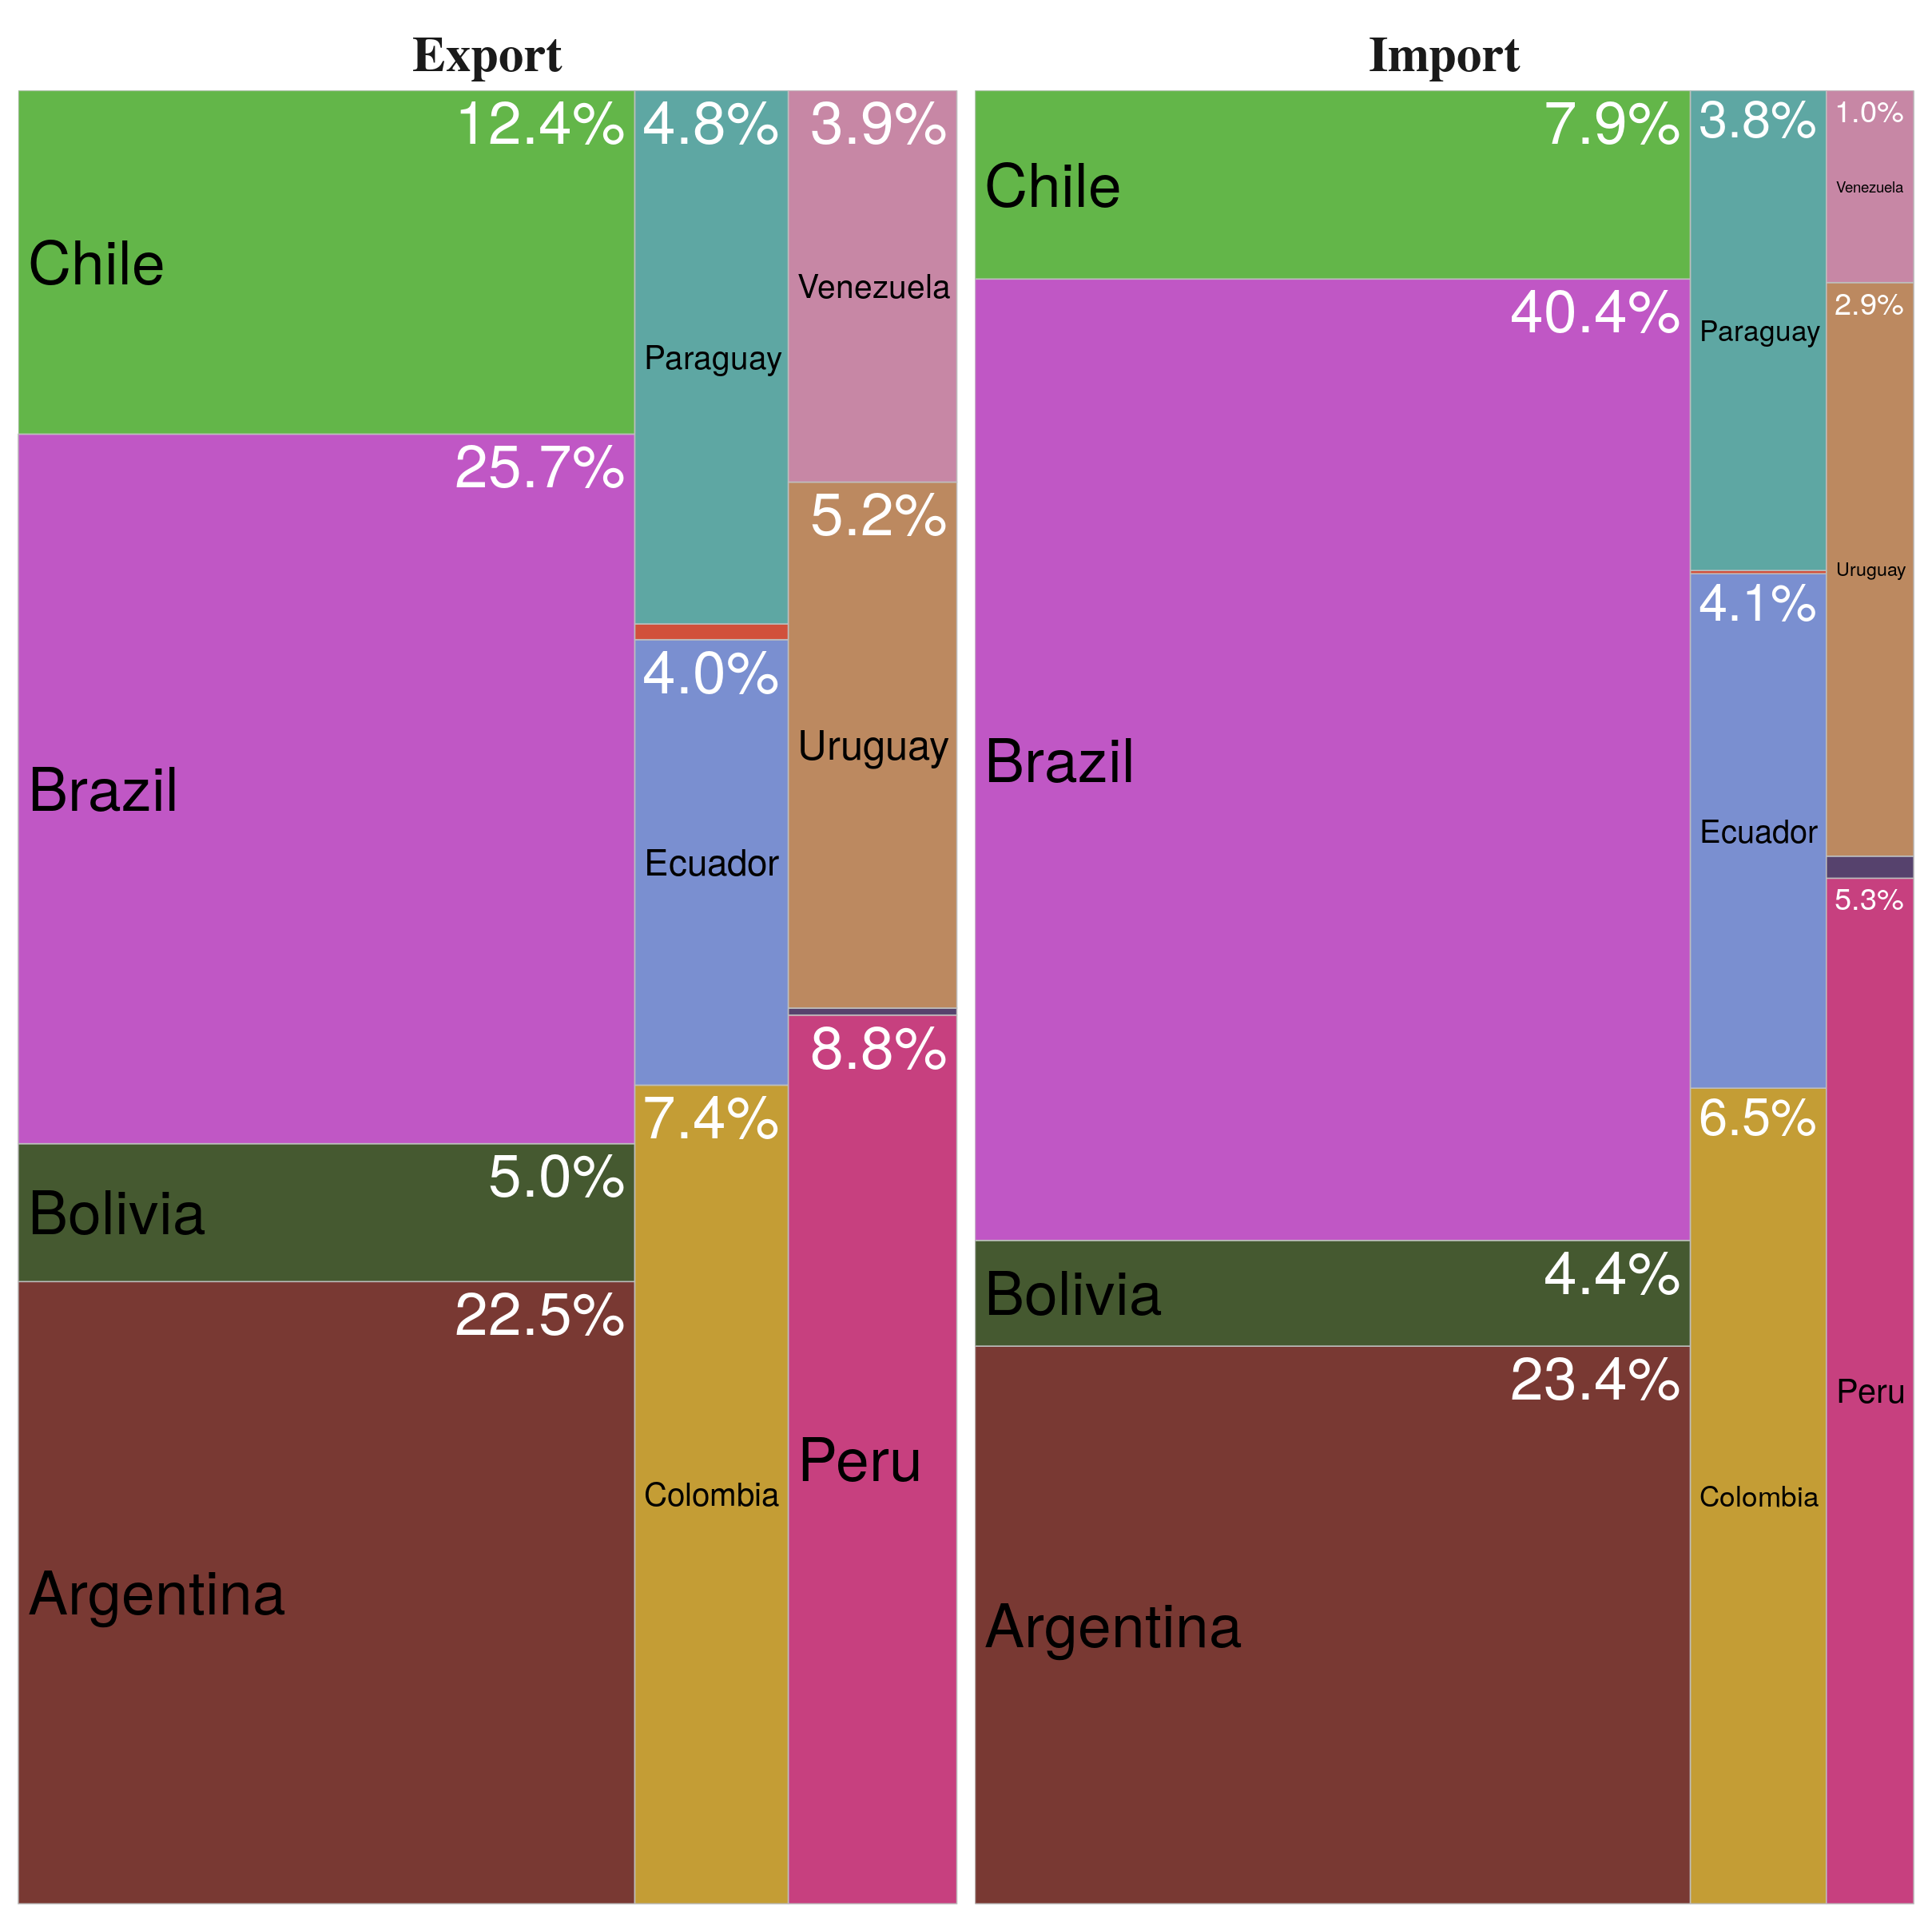
\includegraphics[width=.65\linewidth]{treemaps_paises2016}}
	\subfigure[Incluyendo Resto del mundo]{\label{fig:treemaps_sudamerica_destino_2}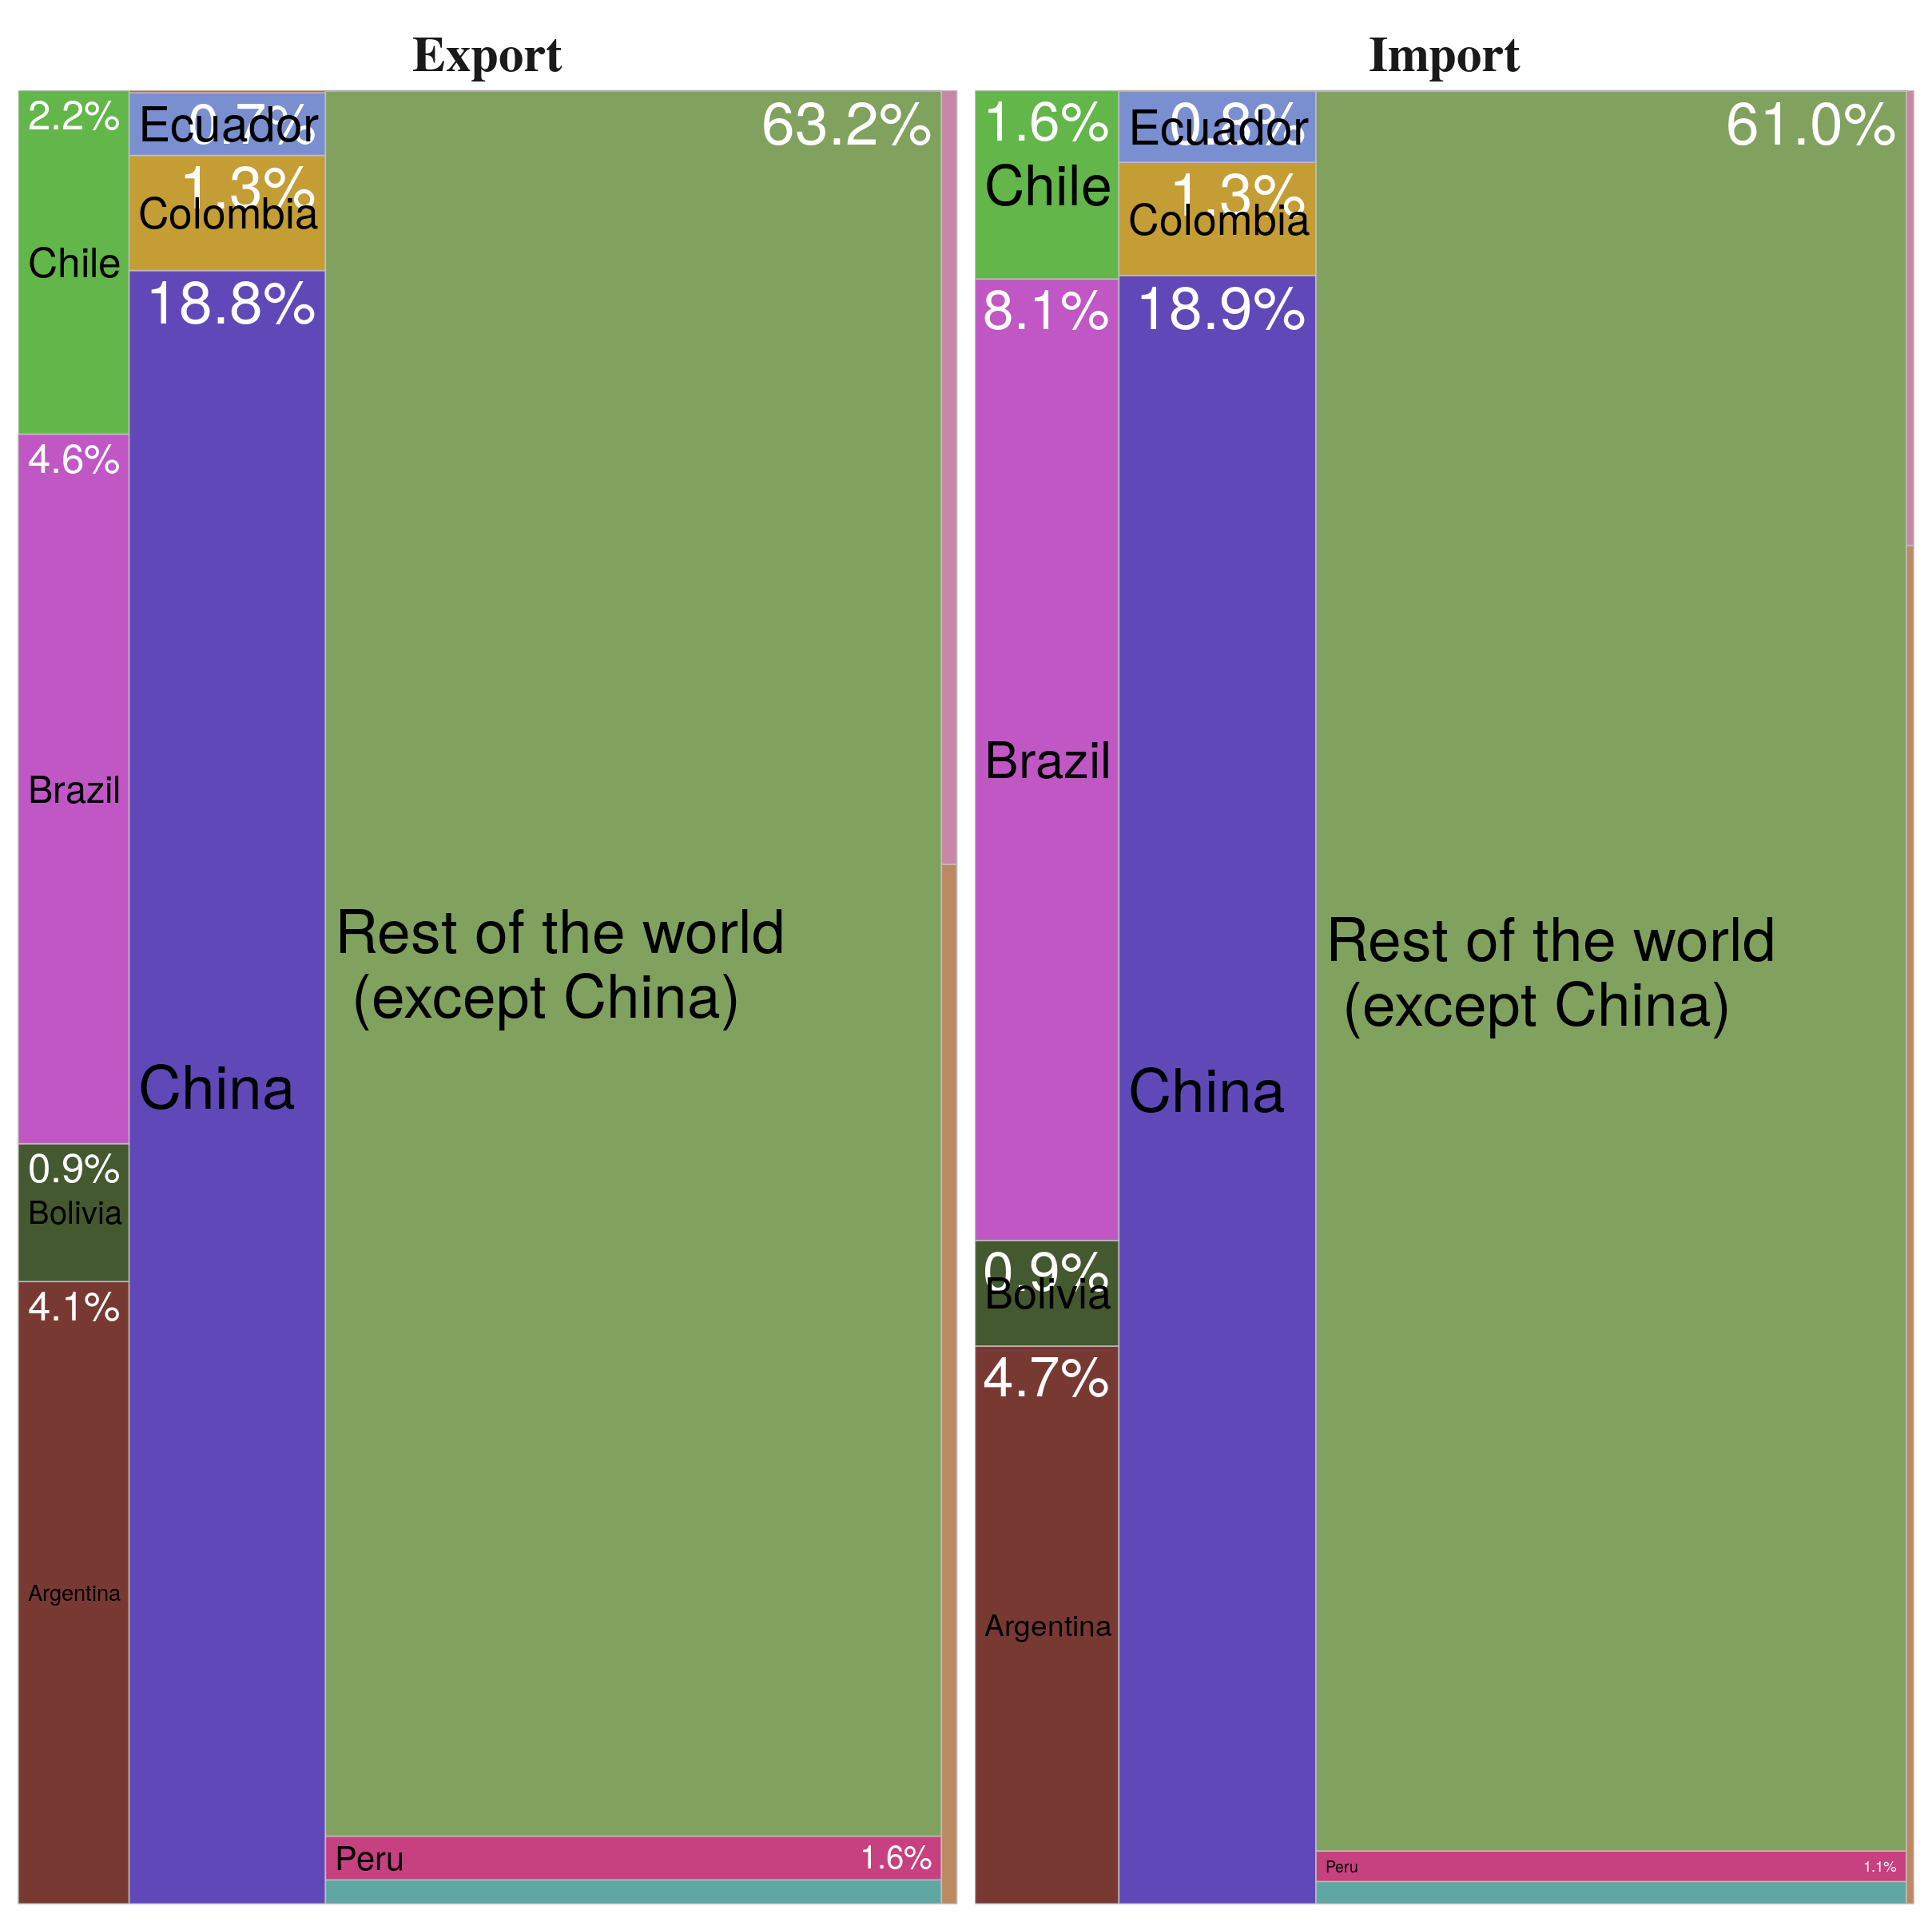
\includegraphics[width=.65\linewidth]{treemaps_paises_rdm2016}}
	\caption{Treemaps según socio comercial. 2016. Total Latinoamérica}
	\label{fig:treemaps_sudamerica_destino}
\end{figure}
	

De las figuras \ref{fig:treemaps_sudamerica_cadsubcad}, \ref{fig:treemaps_sudamerica_usos} y \ref{fig:treemaps_sudamerica_destino} se desprende que la región de Sudamérica tiene una baja integración regional en tanto una pequeña proporción de su comercio se realiza entre países de la región. A su vez, mientras el comercio intrarregional se realiza fundamentalmente sobre productos de alta complejidad y valor agregado, el comercio con el resto del mundo se encuentra desbalanceado: mientras las exportaciones se concentran en productos primarios de baja complejidad, aquellos productos que llegan desde el resto del mundo tienen un mayor grado de tecnificación. Estas conclusiones son particularmente válidas para el comercio con China, que constituye una quinta parte del comercio total de la región. Vale mencionar que la importancia de dicho país ah crecido de forma sostenida en el período analizado, siendo que en 1996 representaba menos de 2\% del comercio \footnote{ver \hyperlink{https://treemaps.shinyapps.io/treemaps/}{https://treemaps.shinyapps.io/treemaps/}}

\section{Metodología}

Del análisis exploratorio se desprende el potencial de la información desagregada a nivel producto para caracterizar la inserción en el mercado mundial de un país o región. Sin embargo, dada la alta cardinalidad de la información y la múltiples dimensiones de estudio, resulta dificultoso su estudio de forma general, sin hacer eje en un determinado país, o sin agregar la información según un nomenclador. En particular, el uso de agrupaciones jerárquicas de los productos resulta esencial para el análisis de resultados. La elaboración de los mismos constituye una extensa tarea por parte de expertos en las temáticas sectoriales de los diferentes tipos de productos, y el nomenclador resultante esta fuertemente determinado por los objetivos con que sera utilizado. Es por ello que en la presente sección se propone una elaboración alternativa de niveles jerárquicos de agrupamiento de productos. 

\info{agregar grafo bipartito}

	
\subsection{Latent Dirichlet Allocation Models}
	
El objetivo de la presente sección es elaborar un agrupamiento automático de los productos, basado en la información disponible. Este problema puede ser concebido desde dos puntos de vista: por un lado, se puede pensar como un problema de \textit{clustering} donde lo que se busca es crear grupos de productos con similares características. Por otro lado, es un problema de reducción de dimensionalidad, donde lo que se busca es encontrar un espacio de menor dimensión al que existen originalmente los datos. Esto sería posible dado que existe la posibilidad de explotar las similitudes y diferencias entre los distintos productos. 

Sin embargo, las técnicas de clustering tradicionales encuentran problemas en espacios de alta dimensionalidad \citep{aggarwal2001surprising}. A su vez, siguiendo el trabajo de \cite{molinari2016especializacion}, se entiende que los grupos no deberían ser excluyentes, dado que un mismo producto puede ser utilizado en diferentes formas, como producto intermedio o final. En este sentido, el problema se puede especificar como de \textit{clustering difuso}.
	
En concreto, la dimensionalidad del problema se puede pensar como el siguiente espacio:

$$
\mathcal{R}^{N*P*Y*2}
$$
Es decir la interacción de $N$ países, $P$ productos, $Y$ años, tanto para las exportaciones como las importaciones.
La propuesta es utilizar la técnica propuesta por \cite{blei2003latent} conocida como \textit{Latent Dirichlet Allocation Models} o \textit{Topic Modeling}. En su versión original, está técnica se propone como una forma de encontrar los tópicos presentes en un corpus, y la distribución de dichos tópicos sobre cada texto. Este problema es análogo al que se busca en el presente trabajo: Allí se busca una dimensión latente de $k$ tópicos, embebidos en un diccionario de alta dimensionalidad (las palabras presentes en el corpus), que se distribuyen a lo largo de los textos que componen dicho corpus. En el presente problema, se busca una dimensión latente de $k$ \textit{componentes}, embebidos en un nomenclador de alta dimensionalidad, que se distribuyen a lo largo de los países. Esta técnica a su vez puede ser pensada como un problema de clustering difuso, en tanto cada palabra (en el contexto original) puede pertenecer a más de un tópico.

A continuación se realizará una descripción del modelo propuesto por \cite{blei2003latent}, adaptado al presente dominio. 
	
\subsubsection{Definiciones}

\begin{itemize}
\item
Un \textbf{\emph{producto}} es la \emph{unidad básica discreta de los
	datos}, se define como un ítem de un nomenclador (SITC). Se representa
como un vector unitario. Definimos el superíndice \(i\) del vector
como el i-ésimo producto del nomenclador y el i-ésimo elemento del
vector. El V-ésimo producto del nomenclador es el vector \(w\), tal
que \(w^v\)=1 y \(w^u\)=0, \(u\neq v\)
\item
Un \textbf{\emph{país}} es una secuencia de \textbf{N} productos,
definido como \(W= (w_1, w_2, ..., w_N)\)
\item
Nuestro \textbf{corpus} es la colección de \textbf{M} países, definido
como \(D = (d_1, d_2,..., d_M)\)
\item
Un \textbf{\emph{componente}} es una dimensión latente sobre el
corpus, y suponemos una cantidad fija \emph{k} de los mismos.
\item
Nuestro objetivo es obtener:
\end{itemize}

\begin{enumerate}
\def\labelenumi{\arabic{enumi}.}
\item
Una distribución de componentes sobre cada país.
\item
Una distribución de los productos sobre los componentes.
\end{enumerate}


\subsubsection{Proceso generativo e inferencial}

Intuitivamente, suponemos el siguiente proceso generativo de datos:

\begin{itemize}
\item
Para cada país del corpus, imaginamos que las exportaciones surgen de
un proceso de dos etapas:

\begin{itemize}
	\item
	Elegimos aleatoriamente una distribución sobre los componentes
	\item
	Para cada dólar exportado:
	
	\begin{itemize}
		\item
		Elegimos aleatoriamente el componente al que pertence, dada la
		distribución definida en el paso anterior
		\item
		Elegimos aleatoriamente un producto de la distribución
		correspondiente a dicho componente
	\end{itemize}
\end{itemize}
\end{itemize}

\begin{enumerate}
\def\labelenumi{\arabic{enumi}.}
\item
Para cada Componente $k \in \{1,2,... K\}$
\end{enumerate}

\begin{itemize}
\item
Generar una distribución sobre los componentes
$\beta \sim Dir_v(\eta)$ con $\eta \in \mathcal{R}_{>0}$ un
parámetro fijo
\end{itemize}

\begin{enumerate}
\def\labelenumi{\arabic{enumi}.}
\setcounter{enumi}{1}
\item
Para cada país $d \in \{1,2,... D\}$
\end{enumerate}

\begin{itemize}
\item
generar un vector de proporciones de componentes
$\theta_d \sim Dir_K(\alpha)$ con $\alpha \in \mathcal{R}_{>0}^K$
un parámetro fijo
\item
Para cada dólar exportado:

\begin{enumerate}
	\def\labelenumi{\roman{enumi}.}
	\item
	generar una asignación del componente $z_{dn} \sim Mult(\theta_d)$
	\item
	asignar el producto $w_{dn} \sim Mult(\beta_{zn})$
\end{enumerate}
\end{itemize}

En la figura \ref{fig:grafo_blei} se puede observar el proceso generativo de forma gráfica. Aquí, cada nodo representa una distribución de probabilidad. Las aristas significan que la distribución de salida definen los parámetros de la distribución de entrada. Los recuadros significan replicación: El recuadro interior representa que el proceso se realiza para cada dólar exportado en el país. El recuadro exterior representa que el proceso se realiza para cada
país en el corpus.


\begin{figure}
	\centering	
	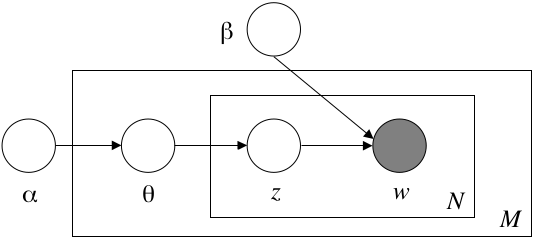
\includegraphics[width=.65\linewidth]{grafo}
	\caption{fuente: \cite{blei2003latent}}
	\label{fig:grafo_blei}
\end{figure}

Un Proceso de Dirichlet es una familia de procesos estocásticos donde las realizaciones son ellas mismas distribuciones de probabilidad. Es decir, el rango de esta distribución (así como en una normal son los reales) son distribuciones de probabilidad. Para interpretarlo geométricamente, la figura \ref{fig:dirichlet} muestra un ejemplo de la distribución de densidad para 3 productos y 4 componentes. El triángulo representa todas las distribuciones (multinomiales)
posibles sobre los tres productos. Cada uno de los vértices del triángulo es una distribución de probabilidad que asigna una probabilidad de 1 a uno de los productos. El punto medio de cada lado, es una distribución con probabilidad 0.5 a dos componentes. El cuarto componente, el centroide del triángulo, asigna probabilidad de $\frac{1}{3}$ a cada producto. Los cuatro puntos marcado con x son las distribuciones multinomiales de $p(w|z)$  para cada uno de los cuatro componentes. La altura en el eje z es una posible distribución de densidad sobre el
simplex, es decir, sobre las distribuciones de densidad multinomiales, dada por LDA.

\begin{figure}
	\centering	
	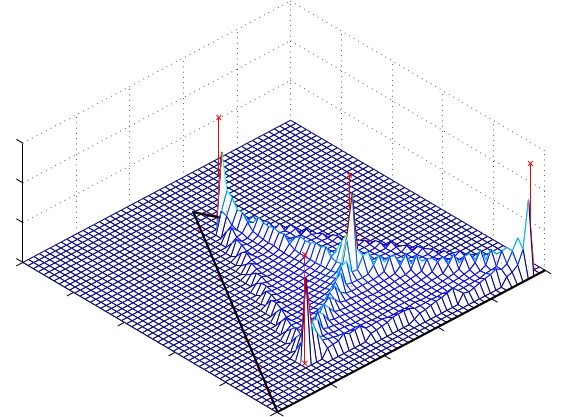
\includegraphics[width=.65\linewidth]{dirichlet}
	\caption{fuente: \cite{blei2003latent}}
	\label{fig:dirichlet}
\end{figure}

Cuando observamos los datos, no contamos con los tópicos ni con su
distribución, sino con los productos y países. El objetivo es realizar
inferencia sobre las variables latentes, mediante el Teorema de Bayes:

$$
p(\theta,z|w,\alpha,\beta) = \frac{p(\theta,z,w|\alpha,\beta)}{p(w|\alpha,\beta)}
$$

Nuestra función objetivo es:

$$
\ell(\alpha, \beta) = \sum_{d=1}^M \log p(w_d|\alpha,\beta)
$$

El problema es que esta ecuación es intratable, por la interacción entre $\theta$ y $\beta$. Por ello, la inferencia se realiza sobre una familia de modelos que se sabe que son una cota inferior de probabilidad, y que son tratables. Estos modelos tienen parámetros variacionales, que se ajustan para obtener el modelo que más se acerca a la cota inferior. La forma de obtener una familia de modelos tratables es considerar algunas modificaciones sobre el modelo gráfico original, removiendo nodos y aristas \citep{hoffman2013stochastic}. En la figura \ref{fig:grafo_variational} se puede observar la solución propuesta por \citep{blei2003latent} que, dado que utilizamos la implementación del modelo que se encuentra en \cite{scikit-learn} es también la del presente trabajo.

\begin{figure}[h]
	\centering	
	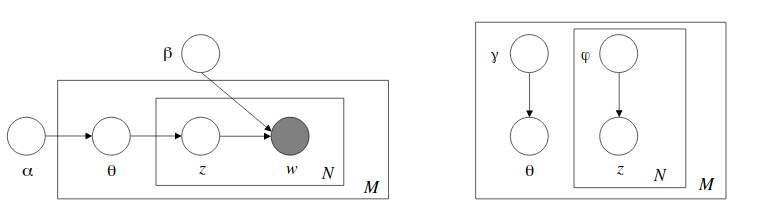
\includegraphics[width=.65\linewidth]{grafo_variational}
	\caption{fuente: \cite{blei2003latent}}
	\label{fig:grafo_variational}
\end{figure}


La estimación de los parámetros se realiza a través del proceso de \emph{variational Expectation Maximization} (EM):

\begin{itemize}
\item \textbf{paso E}: Optimizamos los parámetros variacionales $\gamma, \varphi$
\item \textbf{paso M}: Para los valores fijos $\gamma, \varphi$, maximizamos la cota inferior respecto a los parámetros del modelo, $\alpha,\beta$
\end{itemize}

Estos dos pasos se alternan hasta converger. Por último, se realiza un suavizado sobre las probabilidades que un componente asigna a un producto, para que sean siempre mayores a 0.



\subsection{Grafo Bipartito}
\unsure{ver si llego}

\section{Resultados}

\subsection{Latent Dirichlet Allocation Models}

Los resultado obtenidos de los modelos de Topic Modelling para el análisis de textos normalmente se analizan en dos etapas: En primer lugar se etiquetan los tópicos obtenidos sobre la base de las palabras más salientes de cada tópico, y luego se analiza su distribución en los textos. El etiquetado de los tópicos es una tarea subjetiva donde lo que se busca es un concepto generalizador de aquellas palabras que componen al tópico, donde es posible que esta tarea no se pueda realizar por falta de coherencia dentro del tópico. El hiperparámero $k$, es decir la cantidad de tópicos, juega un rol fundamental en este punto, dado que con una cantidad baja de tópicos estos tenderán a reflejar conceptos amplios, mientras que si $k$ es mayor que la cardinalidad del espacio latente que se busca, esto puede generar tópicos repetidos. 
Lo anterior no escapa al presente dominio sino que se refuerza, dado que la búsqueda, subjetiva, de un concepto abarcador entre productos puede resultar más compleja que la de un concepto generalizador de un grupo de palabras. Un problema que no existe en el presente dominio es el de la polisemia, dado que todos los significantes, indices del nomenclador, hacen referencia a un único significado no ambiguo. Sin embargo, nuevos problemas aparecen respecto a este punto, como qué nomenclador de base utilizar y en qué nivel de desagregación. Por motivos de comparabilidad con los resultados de \cite{molinari2016especializacion} se decidió utilizar el nomenclador SITC a 4 dígitos \citep{un2006standard}. A su vez, se realizaron pruebas para varios valores de $k$: 2,4,6,8,10,20,30,40, 100 y 200. Para el etiquetado de los componentes se observó que la práctica usual de observar los primeros diez elementos de la distribución no bastaba para encontrar una etiqueta generalizadora, por lo que se elaboró un tablero dinámico para estudiar la distribución y su función acumulada, a la vez que se gráfico la distribución en función de un nomenclador de complejidad tecnológica \citep{lall2000technological}: 

\begin{table}[ht]
	\centering
	\begin{tabular}{ll}
		\hline
		 Código & Descripción \\ 
		\hline
		01 & Primary products \\ 
		02 & Resource-based manufactures: agro-based \\ 
		03 & Resource-based manufactures: other \\ 
		04 & Low technology manufactures: textile, garment and footwear \\ 
		05 & Low technology manufactures: other products \\ 
		06 & Medium technology manufactures: automotive \\ 
		07 & Medium technology manufactures: process \\ 
		08 & Medium technology manufactures: engineering \\ 
		09 & High technology manufactures: electronic and electrical \\ 
		10 & High technology manufactures: other \\ 
		99 & Unclassified products \\ 
		\hline
	\end{tabular}
\end{table}

En la figura \ref{fig:dist_40_4} se puede observar la tabla utilizada para caracterizar el cuarto componente en el modelo con $k=4$. Allí se observa que la mayoría de los componentes pertenecen al rubro textil, como pulloveres, remeras y pantalones. También se aparece el té, que no guarda coherencia con le resto del rubro.


\begin{figure}[h]
	\centering	
	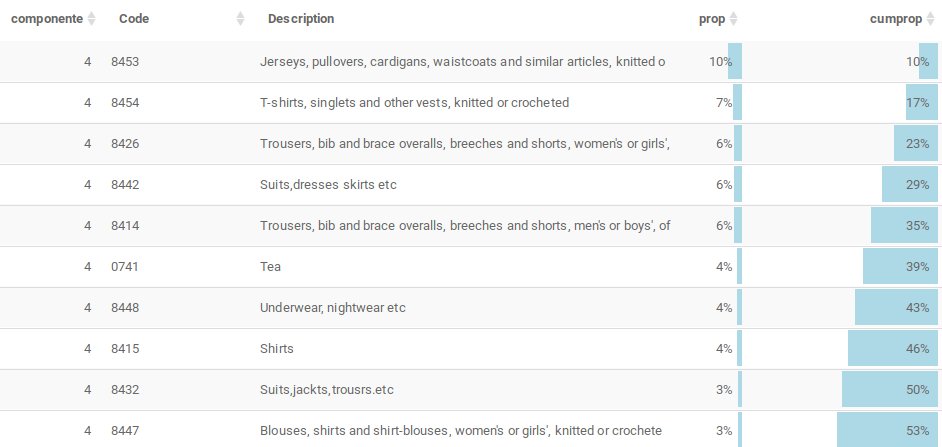
\includegraphics[width=\linewidth]{dist_40_4}
	\caption{Distribución del Componente 4. K = 40}
	\label{fig:dist_40_4}
\end{figure}

La figura muestra la distribución siguiendo los grupos de \cite{lall2000technological}. Aquí se puede confirmar que la distribución se concentra fuertemente en la categoría 4, textiles. 

\begin{figure}[h]
	\centering	
	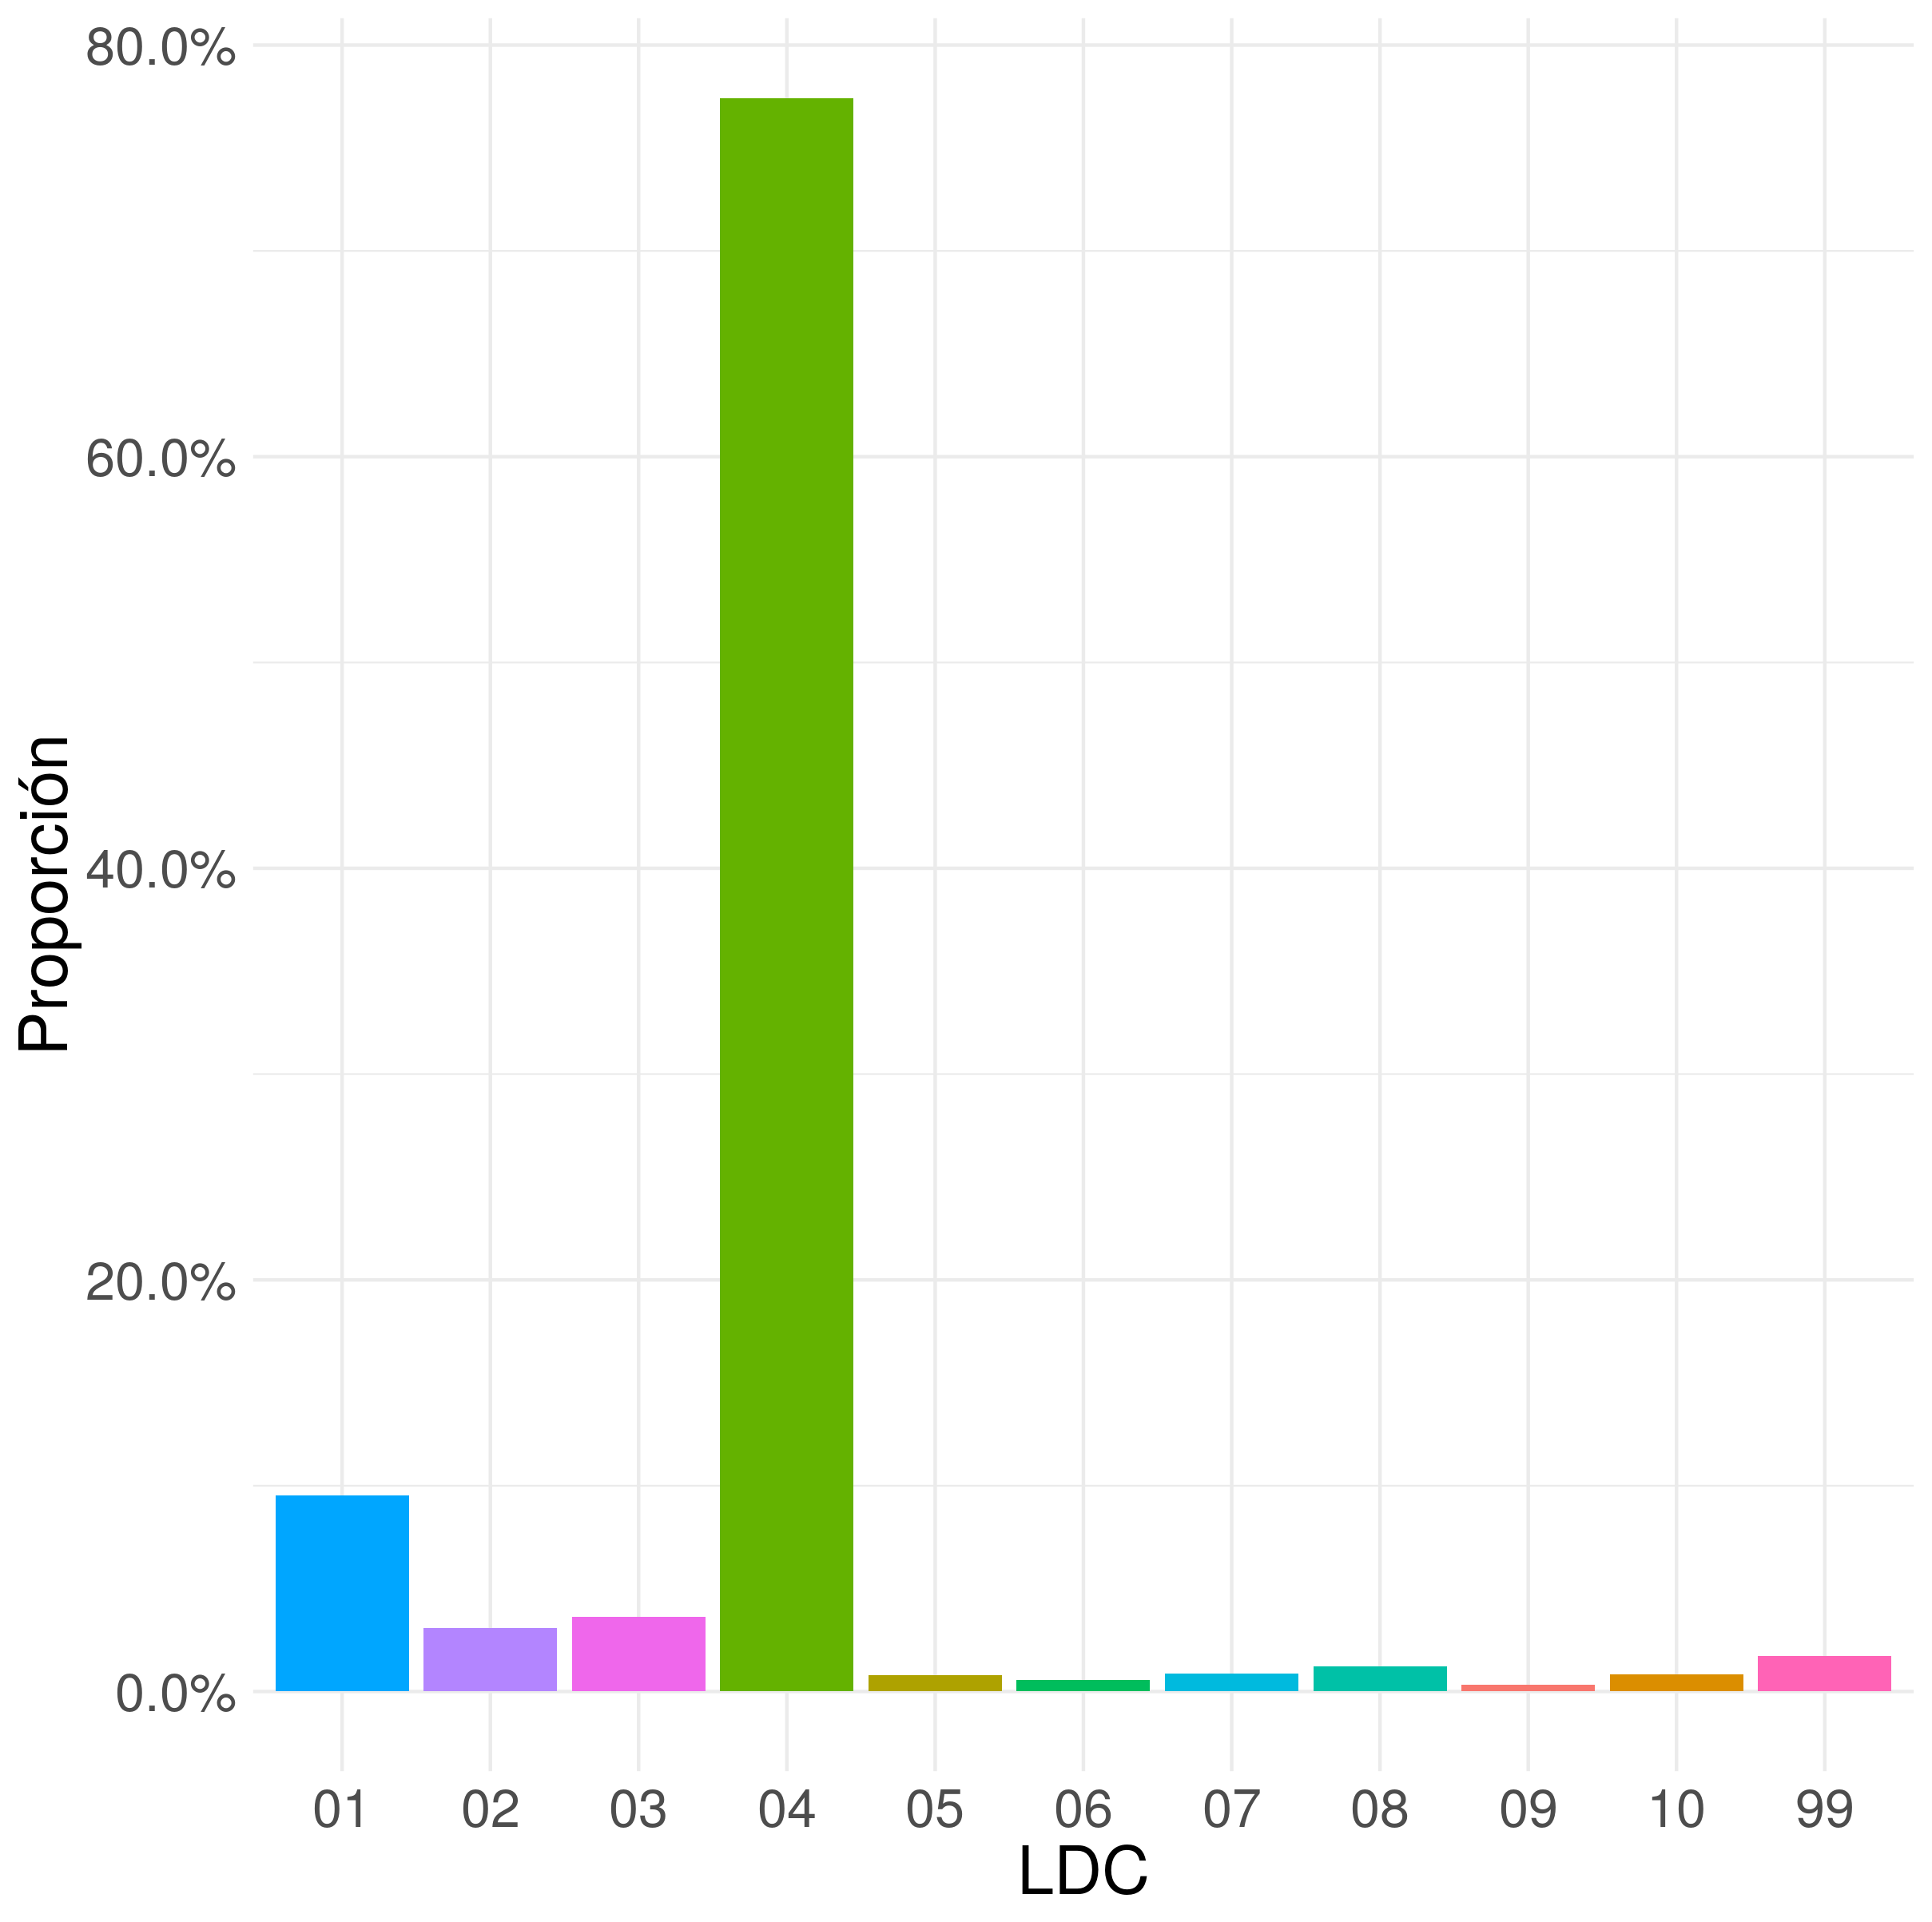
\includegraphics[width=0.65\linewidth]{graficoLall_k40_comp4}
	\caption{Distribución del Componente 4. K = 40 según Lall}
	\label{fig:dist_40_4_lall}
\end{figure}

\info{seguir aca: Granularidad, casos problematicos. 40 es el mejor. Mostrar etiquetas finales.}


\subsection{Grafo Bipartito}
\unsure{ver si llego}



%\bibliographystyle{unsrt}
%\bibliography{bibliografia}
%
\end{document}

